\chapter{硬件平台搭建}
\label{chap:2}
本章主要研究硬件平台的构成及各个传感器数学模型,为后续章节研究VIO算法提供硬件支撑。首先,研究传感器的数学模型以及选型;其次,研究传感器的标定原理及方法,传感器之间的硬件同步方案;最后,研究传感器信息采集方案。
\section{传感器模型与选型}
\subsection{相机及畸变模型}
\label{chap:2.1.1}
(1)针孔相机模型

众所周知,小孔成像能够将3D物体投影成2D图像。相机成像原理类似,称为针孔相机模型。如图\ref{fig2_1}所示。
\begin{figure}[h]\setlength{\belowcaptionskip}{-12pt}
	\centering
	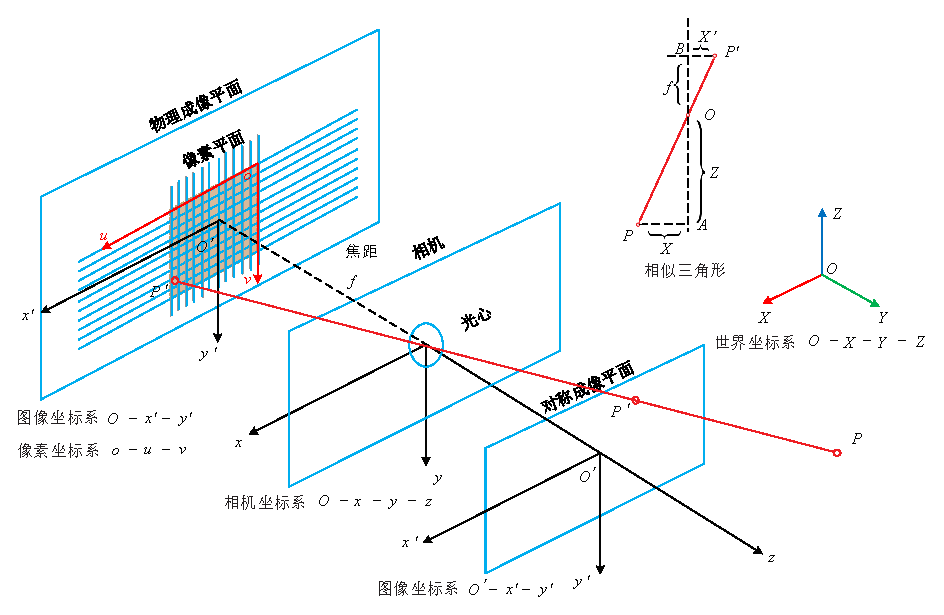
\includegraphics[width=1\textwidth]{figures/chapter2/fig2_1}
	\caption{针孔相机模型}\label{fig2_1}
\end{figure}
其中$O-x-y-z $是相机的坐标系,$z $轴正方向是相机前方,向右为$x $轴正方向,向下为$y $轴正方向。$O $为相机的光心,即针孔模型的针孔。真实世界中三维坐标点$P$,经过光心$O $投影到物理成像平面$O^{\prime}-x^{\prime}-y^{\prime}$上,即图像坐标系,投影坐标点是$P^{\prime} $。设$P$在相机坐标系下的坐标为$[X, Y, Z]^{T} $,$P^{\prime} $ 在图像坐标系下的坐标为$[X^{\prime}, Y^{\prime}]^{T} $ ,光心到物理成像平面的距离为焦距$f$ 。那么,根据相似三角形可得:
\begin{equation}
\label{eqn:2.1}
	\frac{Z}{f}=-\frac{X}{X^{\prime}}=-\frac{Y}{Y^{\prime}}
\end{equation}
其中的负号是因为这个成像看起来是上下颠倒的。为了简化模型,将物理成像平面对称平移到相机的前方,即与三维空间点 $P$ 在同一侧。

这个时候就可以将式(\ref{eqn:2.1})中的负号去掉,得到更加简洁的式子:
\begin{equation}
\label{eqn:2.2}
	\frac{Z}{f}=\frac{X}{X^{\prime}}=\frac{Y}{Y^{\prime}}
\end{equation}
整理得到:
\begin{equation}
\label{eqn:2.3}
	\left\{\begin{aligned} X^{\prime} &=f \frac{X}{Z} \\ Y^{\prime} &=f \frac{Y}{Z} \end{aligned}\right.	
\end{equation}
将成像平面平移到相机前方只是为了简化成像模型,是一种数学手段,不会带来负面影响。所以,在不引起异议的情况下,将这种简化的成像模型定义为针孔模型。

式(\ref{eqn:2.3})建立了三维空间点 和它的二维成像点 之间的映射关系。然而,相机采集的图像是以像素为单位的,所以,为了描述光线到像素之间的映射关系,假设在物理成像平面上固连了一个像素平面 ,如图\ref{fig2_1}所示。

图像的左上角$o $是像素坐标系的原点,向右为$u $轴正方向,向下为$v $轴正方向。设$P^{\prime} $在像素坐标系下的坐标为$[u, v]^{T} $ ,像素坐标在$u $轴上缩放了$\alpha $倍,在$v $轴上缩放了$\beta $倍,原点平移了$\left[c_{x}, c_{y}\right]^{T} $。那么,$P^{\prime} $的图像坐标与像素坐标之间的映射关系为:
\begin{equation}
\label{eqn:2.4}
\left\{\begin{array}{l}{u=\alpha X^{\prime}+c_{x}} \\ {v=\beta Y^{\prime}+c_{y}}\end{array}\right.
\end{equation}
代入式(\ref{eqn:2.3}),得:
\begin{equation}
\label{eqn:2.5}
\left\{\begin{array}{l}{u=f_{x} \frac{X}{Z}+c_{x}} \\ {v=f_{y} \frac{Y}{Z}+c_{y}}\end{array}\right.
\end{equation}
其中,$f_x=\alpha f$ ,$f_y=\beta f  $ 。 $f $ 的单位为米,$\alpha ,\beta $ 得单位为像素每米,$f_x $  和 $f_y $  的单位为像素。通过齐次坐标,将式写成矩阵形式,得:
\begin{equation}
\label{eqn:2.6}
\left( 
\begin{array}{l}{u} \\ {v} \\ {1}\end{array}
\right)=
\frac{1}{Z} \left( 
\begin{array}{ccc}{f_{x}} & {0} & {c_{x}} \\ {0} & {f_{y}} & {c_{y}} \\ {0} & {0} & {1}\end{array}
\right) 
\left( 
\begin{array}{l}{X} \\ {Y} \\ {z}\end{array}
\right) 
\triangleq \frac{1}{Z} \bm{K} \bm{P}
\end{equation}
等式两边同时乘以$Z $得:
\begin{equation}\label{eqn:2.7}
Z \left( \begin{array}{l}{u} \\ {v} \\ {1}\end{array}\right)=\left( \begin{array}{ccc}{f_{x}} & {0} & {c_{x}} \\ {0} & {f_{y}} & {c_{y}} \\ {0} & {0} & {1}\end{array}\right) \left( \begin{array}{l}{X} \\ {Y} \\ {Z}\end{array}\right) \triangleq \bm{K} \bm{P}
\end{equation}
其中,$\bm{K} $ 为相机的内参矩阵,下文中的相机标定需要标定此参数。有时候,为了不失一般性,可以在内参矩阵中添加一个扭曲参数 $\gamma $ ,该参数用来表示像素坐标系的两个坐标轴之间的扭曲程度。此时,内参矩阵$\bm{K} $有5个参数:
\begin{equation}
\label{eqn:2.8}
\bm{K} = \left[\begin{array}{ccc}f_x&\gamma&c_x\\0&f_y&c_y\\0&0&1\end{array}\right]
\end{equation}

值得注意的是,式(\ref{eqn:2.6})中$\bm{P} $ 是点$P $ 在相机坐标系下的坐标。记点$P $在世界坐标系下的坐标为 $\bm{P}_w $ ,则  $\bm{P} $ 和  $\bm{P}_w $ 之间存在一个坐标变换,这个变换矩阵由相机当前的位姿决定。记点$P $在像素坐标系下的坐标为$\bm{P}_{uv} $ ,设相机的旋转和平移为 $\bm{R} $ ,$\bm{t} $ ,那么有:
\begin{equation}
\label{eqn:2.9}
Z \bm{P}_{u v}=Z \left[ \begin{array}{l}{u} \\ {v} \\ {1}\end{array}\right]
=\bm{K}\left(\bm{R} \bm{P}_{w}+\bm{t}\right)=\bm{K} \bm{T} \bm{P}_{w}
\end{equation}
其中,$\bm{T} $为变换矩阵,又叫做特殊欧式群(Special Euclidean Group):
\begin{equation}
\label{eqn:2.10}
S E(3)=\left\{
\bm{T}=\left[ \begin{array}{cc}{\bm{R}} & {\bm{t}} \\ {\bm{0}^{T}} & {1}\end{array}\right] \in \mathbb{R}^{4 \times 4} | 
\bm{R} \in S O(3), \bm{t} \in \mathbb{R}^{3}\right\} 
\end{equation}

式(\ref{eqn:2.9})两侧使用的都是齐次坐标,也就是对相机投影平面进行了归一化,所以式(\ref{eqn:2.9})可以简化为:
\begin{equation}
\label{eqn:2.11}
\boldsymbol{P}_{u v}=\boldsymbol{K} \boldsymbol{T} \boldsymbol{P}_{w}
\end{equation}

式(\ref{eqn:2.11})表达了世界坐标系下的坐标与像素坐标系下的坐标之间的映射关系,也就是所谓的针孔相机模型。

(2)相机畸变模型

上一小节研究的针孔相机模型是理想情况下的模型,实际上,相机的镜头影响光线的传播方向,进而影响成像。影响分为两个方面:一是镜头的形状会对光线产生折射,二是镜头和相机在机械组装时镜头和感光平面不完全平行导致成像的位置发生变化。这两种影响都会使图形产生畸变,前者引起的畸变称为径向畸变,后者引起的畸变称为切向畸变。

图\ref{fig2_2}展示了两种不同类型的径向畸变。
\begin{figure}[h]\setlength{\belowcaptionskip}{-12pt}
	\centering
	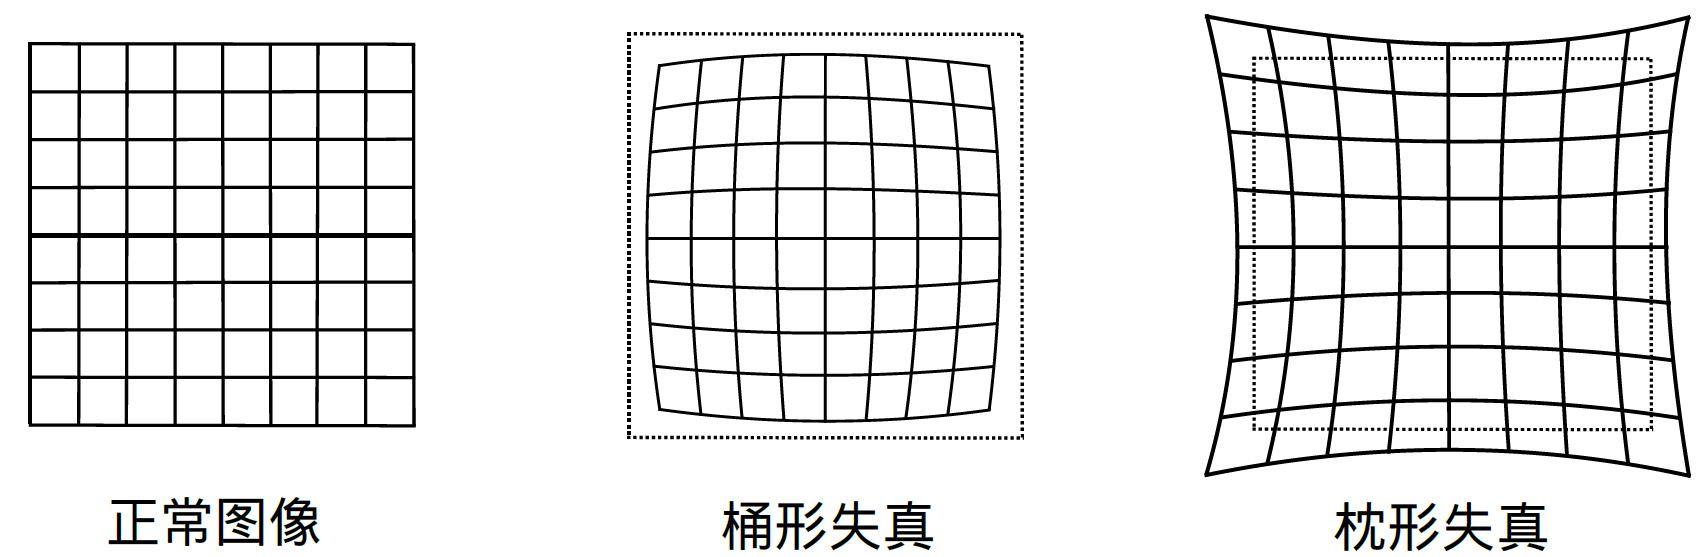
\includegraphics[width=0.7\textwidth]{figures/chapter2/fig2_2}
	\caption{两种类型的径向畸变}\label{fig2_2}
\end{figure}

切向畸变示意图如图\ref{fig2_3}。设归一化成像平面上的点$p $的笛卡尔坐标为 $[x, y]^{T} $ ,极坐标为 $[r, \theta]^{T} $ 。径向畸变使坐标点的长度 $r $ 变化了$\delta r $  ,切向畸变使坐标点的水平夹角 $\theta$ 变化了$\delta \theta $  。
\begin{figure}[h]\setlength{\belowcaptionskip}{-12pt}
	\centering
	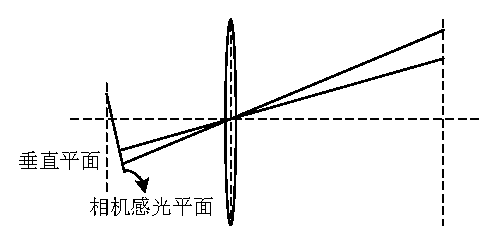
\includegraphics[width=0.5\textwidth]{figures/chapter2/fig2_3}
	\caption{切向畸变示意图}\label{fig2_3}
\end{figure}

使用一个函数来表达径向畸变前后坐标的变化:
\begin{equation}
\label{eqn:2.12}
\left\{\begin{aligned} x_{\text {corrected}} &=x\left(1+k_{1} r^{2}+k_{2} r^{4}+k_{3} r^{6}\right) \\ y_{\text {corrected}} &=y\left(1+k_{1} r^{2}+k_{2} r^{4}+k_{3} r^{6}\right) \end{aligned}\right.
\end{equation}
其中,$\left[x_{\text {corrected }}, y_{\text {corrected}}\right]^{T} $ 表示去畸变后的坐标。公式(\ref{eqn:2.12})中,越靠近图像中心,畸变越小,畸变系数 $k_1$  起主导作用。越远离图像中心,畸变越大,畸变系数 $k_2$ 起主导作用。一般的针孔相机用这两个系数就能去除径向畸变。对于像鱼眼镜头等畸变较大的相机,可以加入 $k_3$  来去畸变。

对于切向畸变,可以使用参数$p_1,p_2$来进行去畸变:
\begin{equation}
\label{eqn:2.13}
\left\{
\begin{aligned} 
x_{\text {corrected}} &=x+2 p_{1} x y+p_{2}\left(r^{2}+2 x^{2}\right) \\ 
y_{\text {corrected}} &=y+p_{1}\left(r^{2}+2 y^{2}\right)+2 p_{2} x y 
\end{aligned}
\right.
\end{equation}

由式(\ref{eqn:2.12})和式(\ref{eqn:2.13})可以得到坐标点在归一化成像平面上去除径向畸变和切向畸变后的正确坐标点:
\begin{equation}
\label{eqn:2.14}
\left\{
\begin{aligned}
x_{\text {corrected}}&=x\left(1+k_{1} r^{2}+k_{2} r^{4}+k_{3} r^{6}\right)+2 p_{1} x y+p_{2}\left(r^{2}+2 x^{2}\right) \\ 
y_{\text {corrected}}&=y\left(1+k_{1} r^{2}+k_{2} r^{4}+k_{3} r^{6}\right)+p_{1}\left(r^{2}+2 y^{2}\right)+2 p_{2} x y
\end{aligned}
\right.
\end{equation}
进一步,通过内参矩阵可以得到去畸变后的像素坐标:
\begin{equation}
\label{eqn:2.15}
\left\{
\begin{aligned}
u_{\text {corrected}}&=f_{x} x_{\text {corrected}}+c_{x} \\ 
v_{\text {corrected}}&=f_{y} y_{\text {corrected}}+c_{y}
\end{aligned}
\right.
\end{equation}
\subsection{IMU状态模型}
四元数可表示为:
\begin{equation}
\setlength{\abovedisplayskip}{6pt}
\setlength{\belowdisplayskip}{6pt}
\label{eqn:2.16}
\mathbf{q}=q_{w}+q_{x} i+q_{y} j+q_{z} k \quad \Leftrightarrow \quad \mathbf{q}=q_{w}+\mathbf{q}_{v}
\end{equation}
其中,$i,j,k$ 是四元数的虚部,满足:
\begin{equation}
\label{eqn:2.17}
\left\{\begin{array}{l}{i^{2}=j^{2}=k^{2}=-1} \\ {i j=k, j i=-k} \\ {j k=i, k j=-i} \\ {k i=j, i k=-j}\end{array}\right.
\end{equation}
也可以用一个四维向量来表示:
\begin{equation}
\label{eqn:2.18}
\mathbf{q} \triangleq \left[ \begin{array}{cc}
{q_{w}} & {\mathbf{q}_{v} }
\end{array}\right] = \left[ \begin{array}{cccc}
{q_{w}} & {q_{x}} & {q_{y}} & {q_{z} } \end{array}\right]^{T}
\end{equation}
设有两个四元数 $\mathbf{p}, \mathbf{q} $ ,那么四元数的运算可表示如下:\\
(1)加法和减法:
\begin{equation}
\label{eqn:2.19}
\mathbf{p} \pm \mathbf{q}=\left[ \begin{array}{c}{p_{w}} \\ {\mathbf{p}_{v}}\end{array}\right] \pm \left[ \begin{array}{c}{q_{w}} \\ {\mathbf{q}_{v}}\end{array}\right]=\left[ \begin{array}{c}{p_{w} \pm q_{w}} \\ {\mathbf{p}_{v} \pm \mathbf{q}_{v}}\end{array}\right]
\end{equation}
满足交换律和结合律,
\begin{equation}
\label{eqn:2.20}
\mathbf{p}+\mathbf{q}=\mathbf{q}+\mathbf{p}
\end{equation}
\begin{equation}
\label{eqn:2.21}
\mathbf{p}+(\mathbf{q}+\mathbf{r})=(\mathbf{p}+\mathbf{q})+\mathbf{r}
\end{equation}
(2)乘法:
\begin{equation}
\label{eqn:2.22}
\mathbf{p} \otimes \mathbf{q}=\left[ \begin{array}{c}{p_{w} q_{w}-p_{x} q_{x}-p_{y} q_{y}-p_{z} q_{z}} \\ {p_{w} q_{x}+p_{x} q_{w}+p_{y} q_{z}-p_{z} q_{y}} \\ {p_{w} q_{y}-p_{x} q_{z}+p_{y} q_{w}+p_{z} q_{x}} \\ {p_{w} q_{z}+p_{x} q_{y}-p_{y} q_{x}+p_{z} q_{w}}\end{array}\right]
\end{equation}
其中, $\otimes$ 表示四元数相乘。写成标量和矢量部分,
\begin{equation}
\label{eqn:2.23}
\mathbf{p} \otimes \mathbf{q}=\left[ \begin{array}{c}{p_{w} q_{w}-\mathbf{p}_{v}^{\top} \mathbf{q}_{v}} \\ {p_{w} \mathbf{q}_{v}+q_{w} \mathbf{p}_{v}+\mathbf{p}_{v} \times \mathbf{q}_{v}}\end{array}\right]
\end{equation}
不满足交换律,
\begin{equation}
\label{eqn:2.24}
\mathbf{p} \otimes \mathbf{q} \neq \mathbf{q} \otimes \mathbf{p}
\end{equation}
满足结合律和分配律,
\begin{equation}
\label{eqn:2.25}
(\mathbf{p} \otimes \mathbf{q}) \otimes \mathbf{r}=\mathbf{p} \otimes(\mathbf{q} \otimes \mathbf{r})
\end{equation}
\begin{equation}
\label{eqn:2.26}
\mathbf{p} \otimes(\mathbf{q}+\mathbf{r})=\mathbf{p} \otimes \mathbf{q}+\mathbf{p} \otimes \mathbf{r} \quad  
\text{and}
\quad(\mathbf{p}+\mathbf{q}) \otimes \mathbf{r}=\mathbf{p} \otimes \mathbf{r}+\mathbf{q} \otimes \mathbf{r}
\end{equation}
两个四元数的乘积可以等效的表示为两个矩阵的乘积,
\begin{equation}
\label{eqn:2.27}
\setlength{\abovedisplayskip}{6pt}
\setlength{\belowdisplayskip}{6pt}
\mathbf{q}_{1} \otimes \mathbf{q}_{2}=\left[\mathbf{q}_{1}\right]_{L} \mathbf{q}_{2} \quad \text { and } \quad \mathbf{q}_{1} \otimes \mathbf{q}_{2}=\left[\mathbf{q}_{2}\right]_{R} \mathbf{q}_{1}
\end{equation}
其中 $\left[\mathbf{q}\right]_{L}$ 和 $\left[\mathbf{q}\right]_{R}$ 分别为,
\begin{equation}
\label{eqn:2.28}
[\mathbf{q}]_{L}=\left[ \begin{array}{cccc}{q_{w}} & {-q_{x}} & {-q_{y}} & {-q_{z}} \\ {q_{x}} & {q_{w}} & {-q_{z}} & {q_{y}} \\ {q_{y}} & {q_{z}} & {q_{w}} & {-q_{x}} \\ {q_{z}} & {-q_{y}} & {q_{x}} & {q_{w}}\end{array}\right], \quad[\mathbf{q}]_{R}=\left[ \begin{array}{cccc}{q_{w}} & {-q_{x}} & {-q_{y}} & {-q_{z}} \\ {q_{x}} & {q_{w}} & {q_{z}} & {-q_{y}} \\ {q_{y}} & {-q_{z}} & {q_{w}} & {q_{x}} \\ {q_{z}} & {q_{y}} & {-q_{x}} & {q_{w}}\end{array}\right]
\end{equation}
或者,
\begin{equation}
\label{eqn:2.29}
[\mathbf{q}]_{L}=q_{w} \mathbf{I}+\left[ \begin{array}{cc}{0} & {-\mathbf{q}_{v}^{\top}} \\ {\mathbf{q}_{v}} & {\left[\mathbf{q}_{v}\right]_{ \times}}\end{array}\right], \quad[\mathbf{q}]_{R}=q_{w} \mathbf{I}+\left[ \begin{array}{cc}{0} & {-\mathbf{q}_{v}^{\top}} \\ {\mathbf{q}_{v}} & {-\left[\mathbf{q}_{v}\right]_{ \times}}\end{array}\right]
\end{equation}
这里,用运算符 $[\bullet]_{\times} $ 产生反对称矩阵,
\begin{equation}
\label{eqn:2.30}
[\mathbf{a}]_{ \times} \triangleq \left[ \begin{array}{ccc}{0} & {-a_{z}} & {a_{y}} \\ {a_{z}} & {0} & {-a_{x}} \\ {-a_{y}} & {a_{x}} & {0}\end{array}\right]
\end{equation}
因为,
\begin{equation}
\label{eqn:2.31}
(\mathbf{q} \otimes \mathbf{x}) \otimes \mathbf{p}=[\mathbf{p}]_{R}[\mathbf{q}]_{L} \mathbf{x} \quad \text { and } \quad \mathbf{q} \otimes(\mathbf{x} \otimes \mathbf{p})=[\mathbf{q}]_{L}[\mathbf{p}]_{R} \mathbf{x}
\end{equation}
所以,
\begin{equation}
\label{eqn:2.32}
[\mathbf{p}]_{R}[\mathbf{q}]_{L}=[\mathbf{q}]_{L}[\mathbf{p}]_{R}
\end{equation}
(3)共轭:
\begin{equation}
\label{eqn:2.33}
\mathbf{q}^{*} \triangleq q_{w}-\mathbf{q}_{v}=\left[ \begin{array}{cc}{q_{w}} & {-\mathbf{q}_{v}}\end{array}\right]^T
\end{equation}
有以下特性,
\begin{equation}
\label{eqn:2.34}
\mathbf{q} \otimes \mathbf{q}^{*}=\mathbf{q}^{*} \otimes \mathbf{q}=q_{w}^{2}+q_{x}^{2}+q_{y}^{2}+q_{z}^{2}=\left[ \begin{array}{c}{q_{w}^{2}+q_{x}^{2}+q_{y}^{2}+q_{z}^{2}} \\ {\mathbf{0}_{v}}\end{array}\right]
\end{equation}
\begin{equation}
\label{eqn:2.35}
(\mathbf{p} \otimes \mathbf{q})^{*}=\mathbf{q}^{*} \otimes \mathbf{p}^{*}
\end{equation}
(4)范数:
\begin{equation}
\label{eqn:2.36}
\|\mathbf{q}\| \triangleq \sqrt{\mathbf{q} \otimes \mathbf{q}^{*}}=\sqrt{\mathbf{q}^{*} \otimes \mathbf{q}}=\sqrt{q_{w}^{2}+q_{x}^{2}+q_{y}^{2}+q_{z}^{2}} \in \mathbb{R}
\end{equation}
(5)逆:
\begin{equation}
\label{eqn:2.37}
\mathbf{q}^{-1}=\mathbf{q}^{*} /\|\mathbf{q}\|^{2}
\end{equation}
\begin{equation}
\label{eqn:2.38}
\mathbf{q} \otimes \mathbf{q}^{-1}=\mathbf{q}^{-1} \otimes \mathbf{q}=\mathbf{q}_{1}
\end{equation}
(6)单位四元数:

对于单位四元数,因为$\|\mathbf{q}\|=1 $ ,所以,
\begin{equation}
\label{eqn:2.39}
\setlength{\abovedisplayskip}{6pt}
\setlength{\belowdisplayskip}{6pt}
\mathbf{q}^{-1}=\mathbf{q}^{*}
\end{equation}
当把单位四元数解释为方向变换或旋转算子时,这个性质意味着可以用共轭四元数实现相反的旋转。单位四元数总是可以写成这种形式,
\begin{equation}
\label{eqn:2.40}
\setlength{\abovedisplayskip}{6pt}
\setlength{\belowdisplayskip}{6pt}
\mathbf{q}=\left[ \begin{array}{cc}{\cos \theta} & {\mathbf{u} \sin \theta}\end{array}\right]^T
\end{equation}
其中,$\mathbf{u}=u_{x} i+u_{y} j+u_{z} k $ 为单位向量, $\theta $为标量。
IMU状态模型主要由运动模型以及观测和噪声模型构成\upcite{sola2017quaternion},状态量包括:$[\mathbf{p}_t, \mathbf{v}_t, \mathbf{q}_t, \mathbf{b}_{a_t}, \bm{b}_{\omega_t},\mathbf{g}^w]$
 ,分别表示 $t$  时刻IMU的位置,速度,姿态(旋转),加速度bias,角速度bias以及世界坐标系下的重力向量。根据式(\ref{eqn:2.22})(\ref{eqn:2.27})(\ref{eqn:2.28})(\ref{eqn:2.29})(\ref{eqn:2.40})可得,
\begin{equation}
\label{eqn:2.41}
\begin{aligned} 
\dot{\mathbf{q}}_{t} &= \lim _{\delta t \rightarrow 0} \frac{1}{\delta t}\left(\mathbf{q}_{t+\delta t}-\mathbf{q}_{t}\right) \\
&= \lim _{\delta t \rightarrow 0} \frac{1}{\delta t}\left(\mathbf{q}_{t} \otimes \delta {\mathbf{q}_{t}}-\mathbf{q}_{t} \otimes \left[ \begin{array}{l}{0} \\ {1}\end{array}\right]\right) \\
&= \lim _{\delta t \rightarrow 0} \frac{1}{\delta t}\left(\mathbf{q}_{t} \otimes \left[ \begin{array}{c}{\mathbf{u} \sin \frac{\theta}{2}} \\ {\cos \frac{\theta}{2}}\end{array}\right]-\mathbf{q}_{t} \otimes \left[ \begin{array}{l}{0} \\ {1}\end{array}\right]\right) \\
& \approx \lim _{\delta t \rightarrow 0} \frac{1}{\delta t} \left( \mathbf{q}_{t} \otimes \left[ \begin{array}{c}{\mathbf{u} \frac{\theta}{2}} \\ {1}\end{array}\right]-\mathbf{q}_{t} \otimes \left[ \begin{array}{l}{0} \\ {1}\end{array}\right] \right) \\
&= \lim _{\delta t \rightarrow 0} \frac{1}{\delta t} \left( \left[ \left[ \begin{array}{c}{\mathbf{u} \frac{\theta}{2}} \\ {1}\end{array}\right]\right]_R-\left[\left[ \begin{array}{l}{0} \\ {1}\end{array}\right]\right]_R \right) \mathbf{\mathbf{q}}_t \\
&= \lim _{\delta t \rightarrow 0} \frac{1}{\delta t} \left[ \begin{array}{cc}{-\frac {[\theta]_{\times}} {2}} & {\frac{\theta}{2}} \\ {-\frac{\theta^{T}}{2}} & {0}\end{array}\right]\mathbf{\mathbf{q}}_t
\end{aligned} 
\end{equation}
其中 $\delta \mathbf{q}_t $ 表示在 $t$  时刻加的三维小扰动。又因为角速度为:
\[
\setlength{\abovedisplayskip}{6pt}
\setlength{\belowdisplayskip}{6pt}
{\omega}=\lim _{\delta t \rightarrow 0} \frac{\theta}{\delta t} 
\]
所以式(\ref{eqn:2.41})可以化简为:
\begin{equation}
\label{eqn:2.42}
\begin{aligned}
\dot{\mathbf{q}}_{t}&=\frac{1}{2} \left[ \begin{array}{cc}{-[\omega]_{\times}} & {\omega} \\ {-\omega^{T}} & {0}\end{array}\right] \mathbf{q}_{t} \\  
&= \frac{1}{2} \bm{\Omega}(\omega) \mathbf{q}_{t} \\
&= \frac{1}{2} {\left[\left[ \begin{array}{l}{\omega} \\ {0}\end{array}\right]\right]}_R \mathbf{q}_{t} \\
&= \frac{1}{2} \left[\mathbf{q}_{t}\right]_L \otimes \left[ \begin{array}{l}{\omega} \\ {0}\end{array}\right]
\end{aligned}
\end{equation}
假设,$\mathbf{a}_t $ 和$\bm{\omega}_t $ 表示IMU真实的加速度和角速率。假设用$\hat{\textbf{a}}_t $ 和 $\hat{\bm{\omega}}_t $表示加速度和角速率的观测值,即传感器读数,测量噪声为$\mathbf{n}_a $ 和$\mathbf{n}_w $ ,那么,
\begin{equation}
\label{eqn:2.43}
\setlength{\abovedisplayskip}{6pt}
\setlength{\belowdisplayskip}{6pt}
\begin{split}
\hat{\textbf{a}}_t&=\textbf{a}_t+{\textbf{b}_a}_t+\textbf{R}_w^t\textbf{g}^w+\textbf{n}_a \\
\hat{\bm{\omega}}_t&=\bm{\omega}_t+\mathbf{b}_{w_t}+\mathbf{n}_w.
\end{split}
\end{equation}
其中$\mathbf{R}_w^t $ 的作用是将重力矢量从世界坐标系下变换到IMU坐标系下。需要注意的是,式(\ref{eqn:2.43})忽略了地球自转角速率$\bm{\omega}_\mathcal{E} $ ,否则将是:$\hat{\bm{\omega}}_t=\bm{\omega}_t+ \mathbf{R}_w^t \bm{\omega}_\mathcal{E} +\mathbf{b}_{w_t}+\mathbf{n}_w $ 。在大多数情况下,不需要考虑地球自转,但是,当使用的IMU传感器分辨率很高,且具有非常小的噪声和bias时, $\bm{\omega}_\mathcal{E} $可能会被传感器测量到( $\bm{\omega}_\mathcal{E} = {15}^{\circ}/h \approx 7.3×10^{-5} rad/s $)。在这种情况下,为了保持IMU误差模型的有效性,在公式中不应该忽略$\bm{\omega}_\mathcal{E} $ 。

由式(\ref{eqn:2.43})可以得到IMU真实的加速度$\mathbf{a}_t $和角速率 $\bm{\omega}_t $:
\begin{equation}
\label{eqn:2.44}
\setlength{\abovedisplayskip}{6pt}
\setlength{\belowdisplayskip}{6pt}
\begin{split}
\textbf{a}_t &=  \hat{\textbf{a}}_t - {\textbf{b}_a}_t - \textbf{R}_w^t\textbf{g}^w - \textbf{n}_a \\
\bm{\omega}_t   &=  \hat{\bm{\omega}}_t  - \mathbf{b}_{w_t} - \mathbf{n}_w.
\end{split}
\end{equation}
IMU的测量值是在IMU自身坐标系下测量得到的,其中包含了重力矢量,并且受到加速度bias、陀螺仪bias以及附加测量噪声的影响。假设加速度计和陀螺仪附加的测量噪声为高斯白噪声,$\mathbf{n}_a\sim\mathcal{N}(0,\bm{\sigma}_a^2) $ ,$\mathbf{n}_w\sim\mathcal{N}(0,\bm{\sigma}_w^2) $ 。加速度计bias和陀螺仪bias被建模为随机游走,随机游走是一个离散模型。将维纳过程(Wiener Process)\upcite{orey1973sample}离散化就是随机游走。而Wiener Process是高斯白噪声的积分,故其导数为高斯分布模型,$\mathbf{n}_{b_a}\sim\mathcal{N}(0,\bm{\sigma}_{b_a}^2) $ ,$\mathbf{n}_{b_w}\sim\mathcal{N}(0,\bm{\sigma}_{b_w}^2) $ 。所以,可得:
\begin{equation}
\label{eqn:2.45}
\setlength{\abovedisplayskip}{6pt}
\setlength{\belowdisplayskip}{6pt}
\dot{\mathbf{b}}_{a_t}=\mathbf{n}_{b_a},\qquad \dot{\mathbf{b}}_{w_t}=\mathbf{n}_{b_w}
\end{equation}
所以,IMU的运动方程为:
\begin{equation}
\label{eqn:2.46}
\left\{
\begin{aligned} \dot{\mathbf{p}}_{t} &=\mathbf{v}_{t} \\ 
\dot{\mathbf{v}}_{t} &=\mathbf{a}_{t} = \hat{\textbf{a}}_t - {\textbf{b}_a}_t - \textbf{R}_w^t\textbf{g}^w - \textbf{n}_a \\ 
\dot{\mathbf{q}}_{t} &=  \frac{1}{2} \bm{\Omega}(\omega) \mathbf{q}_{t} = \frac{1}{2} \bm{\Omega}\left(\hat{\bm{\omega}}_t  - \mathbf{b}_{w_t} - \mathbf{n}_w \right) \mathbf{q}_{t} \\ 
\dot{\mathbf{b}}_{a_t} &=\mathbf{n}_{b_a} \\ 
\dot{\mathbf{b}}_{w_t} &=\mathbf{n}_{b_w} \\ 
\dot{\mathbf{g}}^{w} &=0 \end{aligned}
\right.
\end{equation}
\subsection{磁力计数学模型}
磁力计也叫电子罗盘,能够测量地球磁场分布,进而计算载体的航向信息\upcite{butala2017modeling}。如图\ref{fig2_4}所示,是地球磁场分布图。地球是一个硕大的磁体,磁感线方向从南极到北极。在磁场的南北两极,磁场垂直于水平面,靠近地球赤道,磁场方向平行于水平面。值得注意的是地球磁场的两极和地球地理两极并不完全的重合,他们之间大约有11°的夹角。

地球上某一点的磁场可以用一个矢量 $\mathbf{H} $来表示,矢量$\mathbf{H} $ 的大小和方向分别代表该点磁场的强度和磁场的方向。如图\ref{fig2_5}所示,矢量$\mathbf{H} $ 可以被分解为两个水平分量 $\mathbf{H}_x,\mathbf{H}_y$ ,和一个垂直分量 $\mathbf{H}_z$ 。 $\alpha$是要求的航向角,它是载体当前的正前方与磁北的夹角。航向角的变化值域是0°$\sim $ 360°。
\begin{figure}[h]\setlength{\belowcaptionskip}{-12pt}
	\centering	
	\begin{minipage}[t]{0.35\linewidth}				
		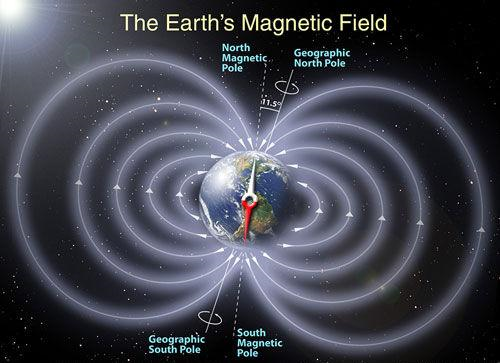
\includegraphics[height=4cm,width=5cm]{figures/chapter2/fig2_4}		
		\caption{地球磁场分布图}	\label{fig2_4}	
	\end{minipage}%	
	\hspace{0.1in}	
	\begin{minipage}[t]{0.5\linewidth}		
		\centering		
		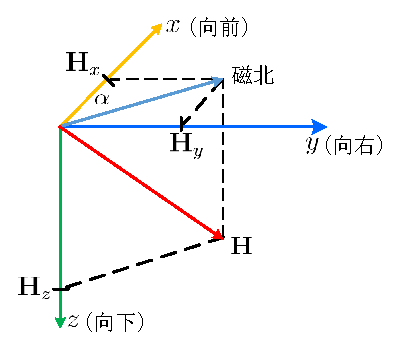
\includegraphics[height=5cm,width=6.5cm]{figures/chapter2/fig2_5}		
		\caption{地磁场矢量分解示意图} \label{fig2_5}		
	\end{minipage}	
\end{figure}
当磁力计水平放置时,磁场矢量$\mathbf{H} $ 在重力方向 $z$ 轴上的分量$\mathbf{H}_z $ 为零,此时$\alpha$ 为:
\begin{equation}
\label{eqn:2.47}
\alpha = \text{arctan}\left(\frac{\mathbf{H}_y}{\mathbf{H}_x}\right)
\end{equation}
但是,通常情况下磁力计不会和水平面完全平行,他们之间会有一个夹角,这个时候就不能通过式(\ref{eqn:2.47})来计算$\alpha$ 的值。需要用加速度计来补偿这个夹角。假设磁力计和加速度计的坐标系重合,在静止或者匀速直线运动的情况下,加速度计测量的三个轴向的加速度是重力加速度在三个轴向的分量。假设在$x,y,z $ 三个轴的测得的重力分量分别为$\mathbf{g}_x, \mathbf{g}_y,\mathbf{g}_z$ ,那么横滚角 $\gamma $和俯仰角$\theta$ 分别为:
\begin{equation}
\label{eqn:2.48}
\begin{aligned}
\gamma &= \text{arctan}\left(\frac{\mathbf{g}_y}{\mathbf{g}_z}\right) \\
\theta &= \text{arcsin}\left( \frac{-\mathbf{g}_x}{\mathbf{g}}\right)
\end{aligned}
\end{equation}
假设磁力计输出的三轴磁分量为$\mathbf{M}_x,\mathbf{M}_y,\mathbf{M}_z $ ,可以根据载体的横滚角 和俯仰角 计算出当地磁场的水平分量$\mathbf{H}_x, \mathbf{H}_y $ :
\begin{equation}
\label{eqn:2.49}
\setlength{\abovedisplayskip}{6pt}
\setlength{\belowdisplayskip}{6pt}
\begin{aligned}
\mathbf{H}_x &= \mathbf{M}_x \text{cos}\theta + \mathbf{M}_y\text{sin}\theta\text{sin}\gamma + \mathbf{M}_z \text{sin}\theta\text{cos}\gamma \\
\mathbf{H}_y &= \mathbf{M}_z\text{sin}\gamma  - \mathbf{M}_y \text{cos}\gamma
\end{aligned}
\end{equation}
将式(\ref{eqn:2.49})代入式(\ref{eqn:2.48})可得航向角 :
\begin{equation}
\label{eqn:2.50}
\alpha = \text{arctan}\left(
\frac{\mathbf{M}_z\text{sin}\gamma  - \mathbf{M}_y \text{cos}\gamma}
{\mathbf{M}_x \text{cos}\theta + \mathbf{M}_y\text{sin}\theta\text{sin}\gamma + \mathbf{M}_z \text{sin}\theta\text{cos}\gamma }\right)
\end{equation}
\subsection{传感器选型}
考虑到本系统的应用环境以及相机和IMU之间需要硬件同步等需求,所以需要慎重选择满足需求的相机和IMU。

(1)单目相机及镜头选型

首先,考虑使用全局快门相机还是卷帘快门相机,这两种相机的成像方式有区别。如图\ref{fig2_6},全局相机是一次性成像,所有像素同时开始和停止曝光,而卷帘相机是逐行成像,每个像素曝光时间不同。因此当拍摄物体运动速度越快,卷帘相机的“果冻效应”就越明显,如图\ref{fig2_7}左图所示。图\ref{fig2_7}右图是的全局快门相机拍摄的图片,可以看到虽然出现了图像模糊问题,但是并没有出现“果冻效应”。对于SLAM系统,高速运动是普遍存在的,因此为了提高系统的鲁棒性,本文选用全局快门相机。其次,对于视觉SLAM系统来说,不需要彩色的图像,利用黑白的图像就可以进行特征点提取与匹配,所以选取灰色相机即可。而且,相机的视角不能太小,太小的话容易导致特征跟踪失败。考虑到室外的环境,相机焦距也不能太短,否则远处的场景会模糊。最后,为了让相机能够在不同的季节和地区正常工作,应该选取具有宽温特性的工业相机。
\begin{figure}[h]\setlength{\belowcaptionskip}{-2pt}
	\centering
	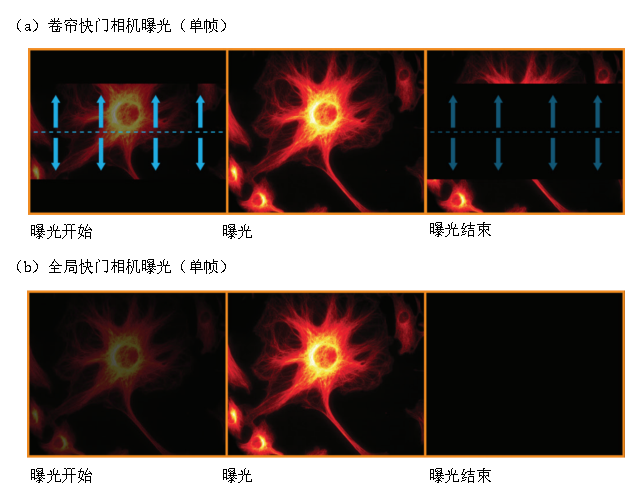
\includegraphics[width=0.7\textwidth]{figures/chapter2/fig2_6}
	\caption{全局相机和卷帘快门相机成像方式}\label{fig2_6}
\end{figure}
\begin{figure}[h]\setlength{\belowcaptionskip}{-12pt}
	\centering
	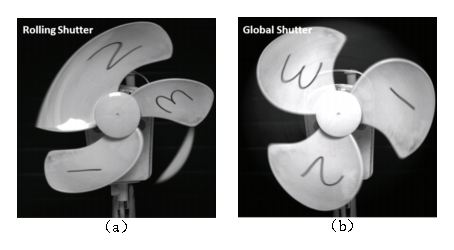
\includegraphics[width=0.5\textwidth]{figures/chapter2/fig2_7}
	\caption{高速运动下的(a)卷帘快门相机图像;(b)全局相机图像}\label{fig2_7}
\end{figure}

基于以上分析,本系统选择灰点公司的Grasshopper3-USB3单目相机,如图\ref{fig2_8}所示。采用快速、高灵敏度的CMOS芯片——IMX174,可提供最高1920×1200的图像分辨率,最高帧率达到163FPS。该相机采用USB 3.0接口,非常适合于处理由传感器产生的远远超过360MByte/s的高速数据传输率,并且比其他高速数字接口更具成本效益。该相机的参数如表\ref{tab2.1}所示。
\begin{figure}[h]\setlength{\belowcaptionskip}{8pt}
	\centering
	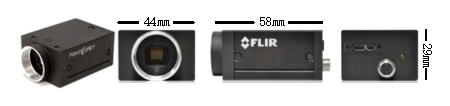
\includegraphics[width=0.7\textwidth]{figures/chapter2/fig2_8}
	\caption{Grasshopper3-USB3相机及其三视图}\label{fig2_8}
\end{figure}
\begin{table}\setlength{\belowcaptionskip}{-12pt}
	\zihao{5}  
	\centering
	\caption{相机参数} \label{tab2.1}
	\begin{tabular}{m{0.15\textwidth}<{\centering} m{0.4\textwidth}<{\centering}}%
		\toprule
		型 \quad\quad 号			&GS3-U3-123S6M-C	 \\
		 \midrule
		分 \ \  辨 \ \  率	       &1920 x 1200         \\
		 \midrule
		帧 \quad\quad 率	    	&163 FPS	         \\
		 \midrule
		传 \ \  感 \ \  器	   &Sony IMX174, CMOS, 1/1.2"	 \\
		 \midrule
		快门方式	              &全局快门             \\
		\midrule
		模数转换                  &10位/12位           \\
		\midrule
		曝光时间                  &0.005 ms ~ 31.9 s   \\
		\midrule
		触发方式                  &Standard, bulb, overlapped, multi-shot \\
		\midrule
		输出格式                  &Mono8, Mono12, Mono16\\
		\midrule
		数据接口                  &USB 3.0                \\
		\midrule
		传输速率                  &5 Gbit/s                \\
		\midrule
		存 \quad\quad 储          &128MB帧缓存,2MB永久闪存    \\
		\midrule
		外观尺寸                  &44 mm×29 mm×58 mm        \\
		\midrule
		重 \quad\quad 量          &90g                    \\
		\midrule
		功 \quad\quad 耗          &≤4.5 W                 \\
		\midrule
		镜头接口                  &C                      \\
		\midrule
		工作温度 	              &0℃~ +50℃               \\
		\bottomrule
	\end{tabular}
\end{table}

相机镜头选用沃乐斯WL1412-1K-1工业定焦镜头,其外观和尺寸如图\ref{fig2_9}所示。表\ref{tab2.2}是沃乐斯WL1412-1K-1镜头参数。
\begin{figure}[!h]\setlength{\belowcaptionskip}{8pt}
	\centering
	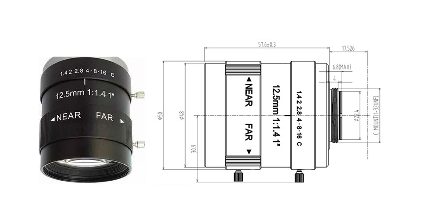
\includegraphics[width=0.45\textwidth]{figures/chapter2/fig2_9}
	\caption{沃乐斯WL1412-1K-1镜头}\label{fig2_9}
\end{figure}
\begin{table}[!h]\setlength{\belowcaptionskip}{-12pt}
	\zihao{5}  
	\centering
	\caption{沃乐斯WL1412-1K-1镜头参数} \label{tab2.2}
	\begin{tabular}{m{0.13\textwidth}<{\centering} m{0.4\textwidth}<{\centering}}%
		\toprule
		型 \quad\quad 号			&GS3-U3-123S6M-C	 \\
		\midrule
		焦 \quad\quad 距	       &1920 x 1200         \\
		\midrule
		接 \quad\quad 口	    	&163 FPS	         \\
		\midrule
		光圈范围	   &Sony IMX174, CMOS, 1/1.2"	 \\
		\midrule
		视 \ \  场\ \  角	              &全局快门             \\
		\midrule
		后 \ \  焦 \ \  距                  &10位/12位           \\
		\midrule
		畸 \ \  变 \ \  率                  &0.005 ms ~ 31.9 s   \\
		\midrule
		分 \ \  辨 \ \  率                  &Standard, bulb, overlapped, multi-shot \\
		\midrule
		外观尺寸                  &Mono8, Mono12, Mono16\\
		\midrule
		工作温度                  &USB 3.0                \\
		\midrule
		重 \quad\quad 量                  &5 Gbit/s                \\
		\bottomrule
	\end{tabular}
\end{table}

(2)IMU选型。

考虑到本系统主要在汽车或无人机上使用,所以光纤陀螺和激光陀螺等大型的高精度惯性器件虽然精度很高,但是通常体积大、重量大,所以不适用于本系统。而MEMS体积小,重量轻,非常适合车载和机载。但是普通的低价MEMS往往精度低,噪声大,会严重影响系统的输出精度。所以,需要尽可能的在成本可接受范围内选择一款相对来说精度高,噪声小,而且具备宽温特性的MEMS。

通过以上分析以及多方对比,本系统的IMU选用挪威Sensonor公司的STIM300。STIM300提供了一个可供外部同步信号输入的IO口和一个与自身采样频率相同的同步方波输出IO口。STIM300及其尺寸图如图\ref{fig2_10}。表\ref{tab2.3}是STIM300的性能参数。
\begin{figure}[!h]\setlength{\belowcaptionskip}{-12pt}
	\centering
	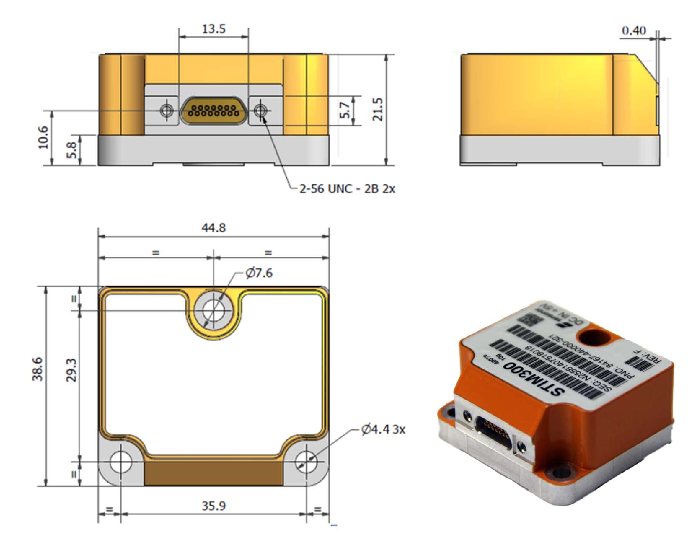
\includegraphics[width=0.6\textwidth]{figures/chapter2/fig2_10}
	\caption{STIM300及其尺寸}\label{fig2_10}
\end{figure}
\begin{table}[!h]
	\zihao{5}  
	\centering
	\caption{STIM300性能参数} \label{tab2.3}
	\begin{tabular}{m{0.13\textwidth}<{\centering} m{0.13\textwidth}<{\centering} m{0.13\textwidth}<{\centering} m{0.13\textwidth}<{\centering} m{0.13\textwidth}<{\centering} m{0.13\textwidth}<{\centering}}%
		\toprule
		\multicolumn{2}{c}{整体指标}  &\multicolumn{2}{c}{陀螺仪性能}       & \multicolumn{2}{c}{加速度计性能}  \\
		\midrule
		重 \quad\quad 量  &	55g	    &测量范围  &	±400°/s	             &测量范围  & ±10g \\
		\midrule
		输出形式          &	RS422     &零\quad\quad 偏  & 0.3°/h           &零\quad\quad 偏  &	0.05mg \\
		\midrule
		工作温度	      & -20℃~ +85℃     &随机游走 & 0.15°/$\sqrt{h}$ 
  &随机游走 & 0.07m/s°/$\sqrt{h}$ \\ 	
		\midrule
		工作电压	      & 5V±0.5V	      &分 \ \  辨 \ \  率   & 0.22°/h	&分 \ \  辨 \ \  率 &	1.9ug \\
		\midrule
		功\quad\quad 耗  & <1.5W	    &全温零偏	   &  ±10°/h rms	   &全温零偏  & ±2mg rms \\
		\midrule
		采样频率  & ≤2kHz & & & & \\
		\bottomrule
	\end{tabular}
\end{table}

值得注意的是,由于本文中视觉/惯性融合系统是紧耦合系统,需要尽可能准确的时间同步,所以需要相机和IMU在硬件上进行同步。这就要求传感器具有触发或者被触发的功能,可以是相机触发IMU,也可以是IMU触发相机。
\section{传感器的标定与同步}
尽管传感器在出厂时已经确定了具体的参数和指标,但是鉴于出厂时不可避免的有安装误差,以及传感器精度会随着使用环境的变化而变化,在使用传感器时有必要对其进行标定。
\subsection{相机标定}
\label{chap:2.2.1}
表\ref{tab2.4} 总结了常见的相机标定方法及其优缺点。
\begin{table}[h]\setlength{\abovecaptionskip}{6pt}
	\zihao{5}  
	\newcommand{\tabincell}[2]{\begin{tabular}{@{}#1@{}}#2\end{tabular}}  %导言区
	\centering
	\caption{常见的相机标定方法及其优缺点} \label{tab2.4}
	\begin{tabular}{m{0.1\textwidth}<{\centering} m{0.2\textwidth}<{\centering} m{0.2\textwidth}<{\centering} m{0.1\textwidth}<{\centering} m{0.1\textwidth}<{\centering}}
		\toprule
		算法分类  &	算法	&   优点   &	缺点   &	标定物  \\
		\midrule
		\multirow{3}*{\tabincell{c}{传统 \\ 标定法} }  & 直接线性变换 (DLT) & \tabincell{c}{模型简单,\\ 计算量小。}&误差较大  & \tabincell{c}{3D立体 \\ 靶标} \\
		\cline{2-5}
		&\tabincell{c}{径向一致约束(RAC)}  & 	\tabincell{c}{标定精度高,\\ 计算量适中。} &	--	 &  \tabincell{c}{3D立体\\靶标} \\
		\cline{2-5}
		&张正友标定法 &	\tabincell{c}{计算量较小,精度 \\ 较高,应用广泛。} &	--   &	\tabincell{c}{2D棋盘格\\标定板}\\
		\midrule
		\tabincell{c}{主动视觉\\标定法}&基于纯旋转的标定 &\tabincell{c}{方法简单,\\鲁棒性高。} &\tabincell{c}{成本高,\\要求高。} & 无标定物 \\
		\midrule
		自标定法 & Kruppa方程标定法 &\tabincell{c}{方法简单,\\灵活性强。} &\tabincell{c}{精度较差,\\计算量大}& 无标定物\\			
		\bottomrule
	\end{tabular}
\end{table}
其中使用最广泛的“张正友标定法” \upcite{zhang2000flexible},该方法优点多,所以采用此方法标定相机参数。

“张正友标定法”使用的标定物是2D棋盘格,如图\ref{fig2_11}所示。由\ref{chap:2.1.1}小节的针孔相机模型可知,标定用的棋盘格平面到像素平面的单应性关系为:
\[
\setlength{\abovedisplayskip}{6pt}
\setlength{\belowdisplayskip}{6pt}
\boldsymbol{P}_{u v}=\boldsymbol{K} \boldsymbol{T} \boldsymbol{P}_{w}
\]
其中,$\bm{P}_w $  为世界坐标点,$\bm{P}_w = [X,Y,Z]^T$ , $\bm{P}_{uv} $ 为像素坐标点,$\bm{P}_{uv} = [u,v]^T$ 。
令$\bm{T}=[ \bm{r}_1, \bm{r}_2, \bm{r}_3, \bm{t}] $  ,棋盘格所在平面为 $Z=0 $  的平面,则,
\begin{figure}[h]\setlength{\belowcaptionskip}{-12pt}
	\centering
	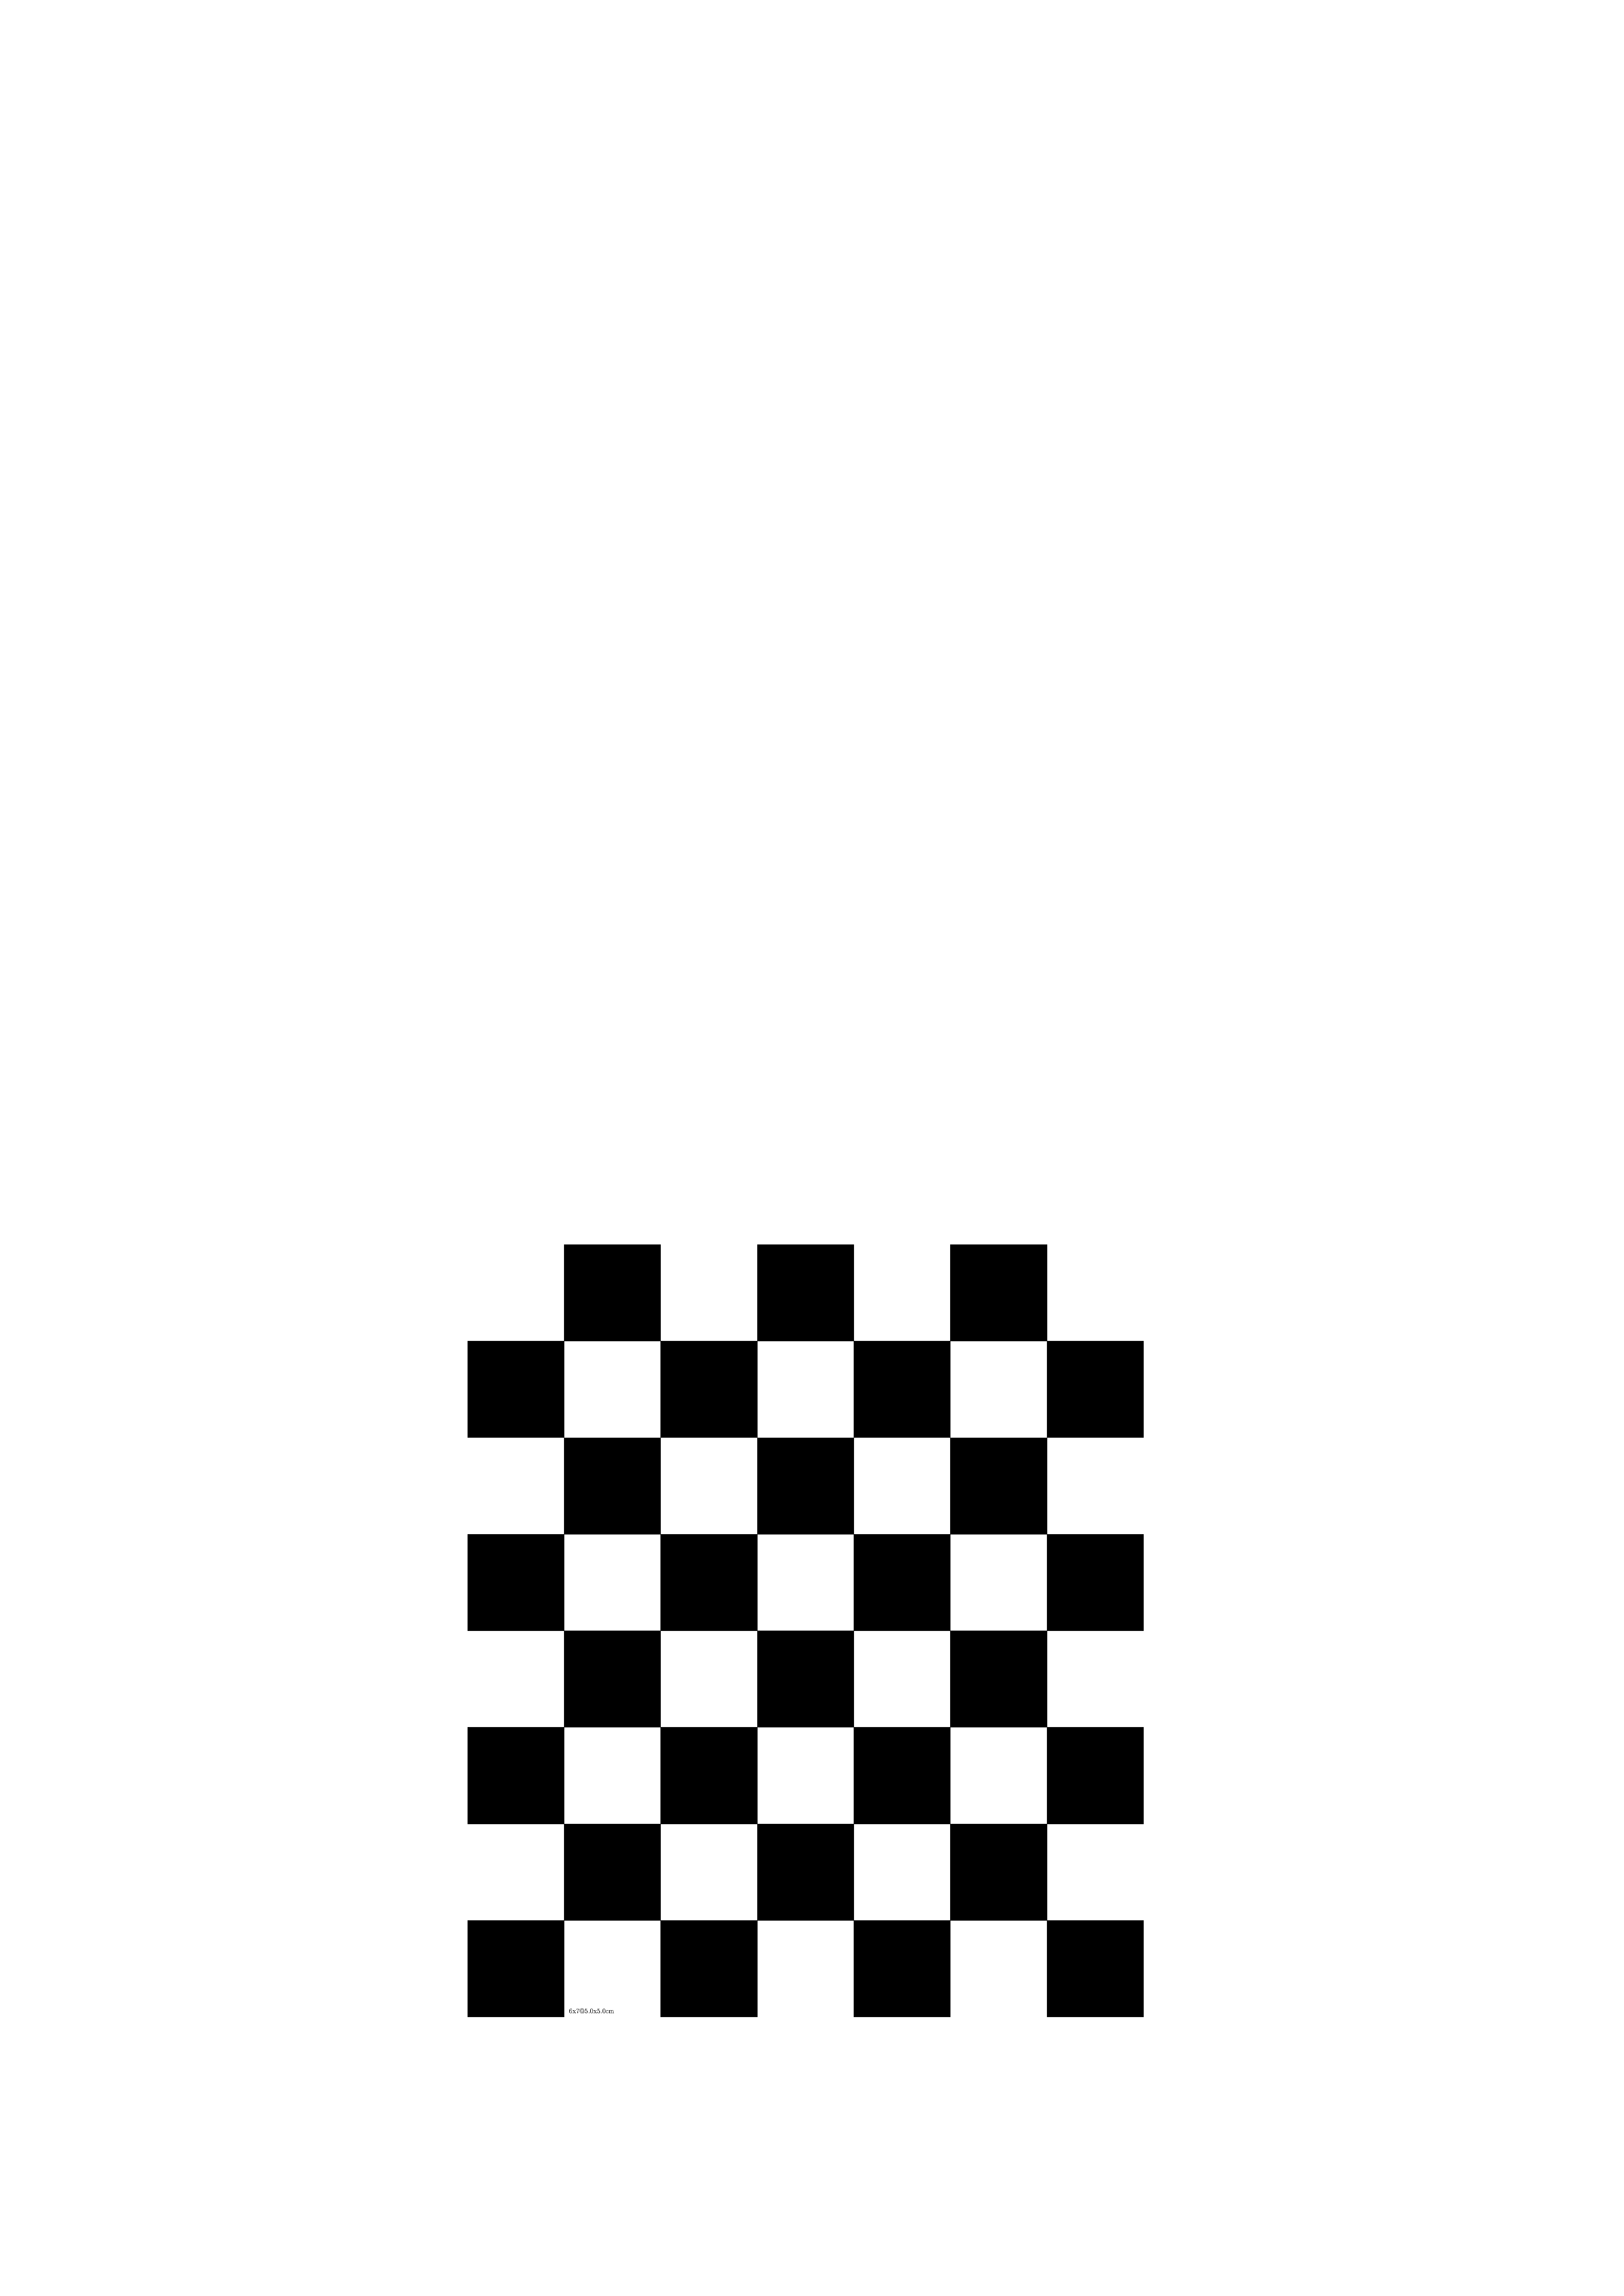
\includegraphics[width=0.2\textwidth]{figures/chapter2/fig2_11}
	\caption{7×6棋盘格}\label{fig2_11}
\end{figure}
\begin{equation}
\label{eqn:2.51}
\begin{aligned}
	s \left[ \begin{array}{c}{u} \\ {v} \\ {1}\end{array}\right] 
	&= \bm{K} \left[ \begin{array}{llll}{\bm{r}_{1}} & {\bm{r}_{2}} & {\bm{r}_{3}} & \bm{t}\end{array}\right] \left[ \begin{array}{c}{X} \\ {Y} \\ {0} \\ {1}\end{array}\right]
	= \bm{K} \left[ \begin{array}{lll}{\bm{r}_{1}} & {\bm{r}_{2}} & \bm{t}\end{array}\right] \left[ \begin{array}{c}{X} \\ {Y} \\ {1}\end{array}\right] \\
	&= \bm{H} \left[ \begin{array}{c}{X} \\ {Y} \\ {1}\end{array}\right] 
\end{aligned}
\end{equation}
其中 $s $是尺度因子, $\bm{H} $是单应矩阵$\bm{H}=\bm{K} \left[ \begin{array}{lll}{\bm{r}_{1}} & {\bm{r}_{2}} & \bm{t}\end{array}\right]  $ 。

$\bm{H} $ 矩阵有八个未知数,棋盘格的每对对应角点能提供两个方程,因此至少需要四个对应角点就可以算出世界平面到像素平面的映射矩阵,即单应矩阵$\bm{H} $ 。

设$\bm{H}=[ \bm{h}_1 \quad \bm{h}_2 \quad  \bm{h}_3 ]=\lambda \bm{K}[ \bm{r}_1 \quad \bm{r}_2 \quad  \bm{t} ] $ ,由式(\ref{eqn:2.51})得,
\begin{equation}
\label{eqn:2.52}
\left\{
\begin{aligned}
\lambda &= \frac{1}{s} \\ 
\bm{r}_{1} &= \frac{1}{\lambda} \bm{K}^{-1} \bm{h}_{1} \\ 
\bm{r}_{2} &= \frac{1}{\lambda} \bm{K}^{-1} \bm{h}_{2}
\end{aligned}
\right.
\end{equation}
因为 $\bm{r}_1 $和$\bm{r}_2 $ 是旋转矩阵,所以  $\bm{r}_1 $和$\bm{r}_2 $ 正交,则
\begin{equation}
\label{eqn:2.53}
\left\{
\begin{aligned}
\bm{r}_{1}^{T} \bm{r}_{2}&=0 \\ 
\left\|\bm{r}_{1}\right\|&=\left\|\bm{r}_{2}\right\|=1
\end{aligned}
\right.
\end{equation}
由式(\ref{eqn:2.52})和(\ref{eqn:2.53})可得,
\begin{equation}
\label{eqn:2.54}
\left\{
\begin{aligned} 
\bm{h}_{1}^{T} \bm{K}^{-T} \bm{K}^{-1} \bm{h}_{2} &=0 \\ 
\bm{h}_{1}^{T} \bm{K}^{-T} \bm{K}^{-1} \bm{h}_{1} &=\bm{h}_{2}^{T} \bm{K}^{-T} \bm{K}^{-1} \bm{h}_{2}=1
\end{aligned}
\right.
\end{equation}

即一个单应性矩阵可以提供两个方程,内参矩阵中有5个参数,因此至少需要3个单应性矩阵才能求解内参矩阵 $\bm{K} $ 。所以至少需要在3个不同的位置拍3张图片才能完成标定任务。

为了便于计算,令
\begin{equation}
\label{eqn:2.55}
\begin{aligned}
\bm{B} &= \bm{K}^{-T}\bm{K}^{-1}
=\left[
\begin{array}{ccc}
B_{11} & B_{12} & B_{13} \\
B_{21} & B_{22} & B_{23} \\
B_{31} & B_{32} & B_{33}
\end{array}
\right]  \\
&=\left[
\begin{array}{ccc}
\frac{1}{\alpha^2} & -\frac{\gamma}{\alpha^2\beta} & \frac{v_0\gamma-u_0\beta}{\alpha^2\beta} \\
-\frac{\gamma}{\alpha^2\beta} & \frac{\gamma^2}{\alpha^2\beta^2}+\frac{1}{\beta^2} & -\frac{\gamma(v_0\gamma-u_0\beta)}{\alpha^2\beta^2}-\frac{v_0}{\beta^2} \\
\frac{v_0\gamma-u_0\beta}{\alpha^2\beta} & -\frac{\gamma(v_0\gamma-u_0\beta)}{\alpha^2\beta^2}-\frac{v_0}{\beta^2} & \frac{(v_0\gamma-u_0\beta)^2}{\alpha^2\beta^2}+\frac{v_0}{\beta^2}+1
\end{array}
\right]
\end{aligned}
\end{equation}
注意,$\bm{B}$是一个对称矩阵,其有效元素为6个,将这6个元素写成向量的形式,
\begin{equation}
\label{eqn:2.56}
\setlength{\abovedisplayskip}{6pt}
\setlength{\belowdisplayskip}{6pt}
\bm{b} =\left[\begin{array}{ccc}B_{11} ,B_{12} , B_{22},B_{13},B_{23},B_{33}\end{array}\right]
\end{equation}
令$\bm{h}_i $ 为 $\bm{H} $的第 $i$  个列向量,则 
\begin{equation}
\label{eqn:2.57}
\setlength{\abovedisplayskip}{6pt}
\setlength{\belowdisplayskip}{6pt}
\bm{h}_i = [h_{i1},h_{i2},h_{i3}]^T
\end{equation}
所以,
\begin{equation}
\label{eqn:2.58}
\bm{h}_i \bm{K}^{-T}\bm{K}^{-1} \bm{h}_j = \bm{h}_i \bm{B} \bm{h}_j = \bm{v}_{ij}^T \bm{b}
\end{equation}
其中,
\[
\setlength{\abovedisplayskip}{6pt}
\setlength{\belowdisplayskip}{6pt}
\begin{aligned}
\bm{v}_{ij} = 
& \left[ \begin{array}{cccccc} 
h_{i1}h_{j1} & h_{i1}h_{j2}+h_{i2}h_{j1} & h_{i2}h_{j2} & h_{i3}h_{j1}+h_{i1}h_{j3} & h_{i3}h_{j2}+h_{i2}h_{j3} & h_{i3}h_{j3} 
\end{array} \right]^T
\end{aligned}
\]
进一步,由式(\ref{eqn:2.51})可推得,
\begin{equation}
\label{eqn:2.59}
\left\{
\begin{aligned} 
\bm{v}_{22}^T \bm{b} &= 0 \\ 
\bm{v}_{11} \bm{b} &= \bm{v}_{12} \bm{b} 
\end{aligned}
\right.
\end{equation}
写成矩阵形式,
\begin{equation}
\label{eqn:2.60}
\left[ 
\begin{array}{c} \bm{v}_{12}^T \\ \bm{v}_{11}-\bm{v}_{22} \end{array}
\right] \bm{b}  = 0
\end{equation}
这是一张棋盘格图像得到的约束等式,当有 $n$  张图像时,
\begin{equation}
\label{eqn:2.61}
\setlength{\abovedisplayskip}{6pt}
\setlength{\belowdisplayskip}{6pt}
\bm{Vb} = 0
\end{equation}
其中,$\bm{V} $ 是一个 $2n \times 6 $的矩阵, $\bm{b} $ 是一个6维列向量,所以,当有三张或者三张以上棋盘格图像时,就可以计算得到$\bm{B} $ ,进而得到相机的内参数矩阵 $\bm{K} $。

以上结果是在理想情况下推导得出的,但是现实中往往存在高斯噪声,所以为了增加标定结果的可靠性,使用MLE(Maximum Likelihood Estimation)来优化上面计算的结果。假设相机从不同的角度采集了$n$ 张包含棋盘格的图像,每张图像里有$m$ 个棋盘格角点。设第$i$ 张图像上的第 $j$个角点的三维点为$\bm{M}_{ij} $ ,则	
\begin{equation}
\label{eqn:2.62}
\setlength{\abovedisplayskip}{6pt}
\setlength{\belowdisplayskip}{6pt}
\hat{m}( \bm{K},\bm{R}_i,\bm{t}_i,\bm{M}_{ij}) = \bm{K}\bm{T}\bm{M}_{ij}
\end{equation}
其中,$\hat{m}( \bm{K},\bm{R}_i,\bm{t}_i,\bm{M}_{ij} )  $ 表示$\bm{M}_{ij} $ 对应的图像角点, $\bm{R}_i,\bm{t}_i $表示相机拍摄第  $i$ 张图像时的旋转和平移,$\bm{K} $ 是相机内参矩阵,角点$m_{ij} $ 的概率密度函数是:
\begin{equation}
\label{eqn:2.63}
f(m_{ij})=\frac{1}{\sqrt{2\pi}}e^{\frac{-(\hat{m}( \bm{K},\bm{R}_i,\bm{t}_i,\bm{M}_{ij} )^2}{\sigma^2}}
\end{equation}
构造似然函数:
\begin{equation}
\label{eqn:2.64}
L(\bm{K},\bm{R}_i,\bm{t}_i,\bm{M}_{ij}  ) = \prod^{n,m}_{i=1,j=1}f(m_{ij})=\frac{1}{\sqrt{2\pi}}e^{\frac{-\sum^n_{i=1}\sum^m_{j=1}(\hat{m}( \bm{K},\bm{R}_i,\bm{t}_i,\bm{M}_{ij} )^2}{\sigma^2}}
\end{equation}
让$L $ 取得最大值,需要最小化下面的式子:
\begin{equation}
\label{eqn:2.65}
\sum^n_{i=1}\sum^m_{j=1} \| \hat{m}( \bm{K},\bm{R}_i,\bm{t}_i,\bm{M}_{ij} )-m_{ij} \|^2
\end{equation}
针对这个最优解问题,可以使用LM(Levenberg-Marquardt)方法\upcite{more1978levenberg}求。

值得注意的是,“张正友标定法”只考虑了影响最大的径向畸变,且只用了前两个畸变参数,即式(\ref{eqn:2.12})中的 $k_1,k_2 $,
\begin{equation}
\label{eqn:2.66}
\left\{
\begin{aligned}
\hat{x} &= x + x[k_1(x^2 + y^2) + k_2(x^2 + y^2)^2] \\
\hat{y} &= y + y[k_1(x^2 + y^2) + k_2(x^2 + y^2)^2]
\end{aligned}
\right.
\end{equation}
其中, $(x,y)$和$(\hat{x},\hat{y}) $ 分别是畸变前和畸变后归一化成像平面的坐标。

设 $(u,v)$和$(\hat{u},\hat{v}) $ 分别是畸变前和畸变后的像素坐标,式(\ref{eqn:2.8})中的 $\gamma = 0 $ ,则,
\begin{equation}
\label{eqn:2.67}
\left\{
\begin{aligned}
\hat u &= u + (u-c_x)[k_1(x^2+y^2)+k_2(x^2+y^2)^2] \\
\hat u &= u + (u-c_y)[k_1(x^2+y^2)+k_2(x^2+y^2)^2]
\end{aligned}
\right.
\end{equation}
将式(\ref{eqn:2.67})写成矩阵形式:
\begin{equation}
\label{eqn:2.68}
\left[
\begin{array}{cc}
(u-c_x)(x^2+y^2) & (u-c_x)(x^2+y^2)^2 \\
(v-c_y)(x^2+y^2) & (v-c_y)(x^2+y^2)^2
\end{array}
\right]
\left[
\begin{array}{c}
k_1 \\ k_2
\end{array}
\right]=
\left[
\begin{array}{c}
\hat u -u \\ \hat v -v
\end{array}
\right]
\end{equation}

式(\ref{eqn:2.68})是从一张图像上的一个角点得到的,假设相机从不同的角度采集了 $n$ 张包含棋盘格的图像,每张图像里有 $m$个棋盘格角点,那么总共可以得到 $2mn$个等式,记作,
\begin{equation}
\label{eqn:2.69}
\bm{Dk} = \bm{d}
\end{equation}
可以得到,
\begin{equation}
\label{eqn:2.70}
\bm{k}=[k_1\ k_2]^T = (\bm{D}^T \bm{D})^{-1} \bm{D}^T\bm{d}
\end{equation}
同样,使用最大似然估计求最优解,使用LM方法最小化下面的式子求取参数,
\begin{equation}
\label{eqn:2.71}
\sum^n_{i=1}\sum^m_{j=1} \| \hat{m}( \bm{K},\bm{k},\bm{R}_i,\bm{t}_i,\bm{M}_{ij}  )-m_{ij} \|^2
\end{equation}

本系统使用的灰点相机标定出的内参和畸变结果如下:
\[
\bm{K}=
\left[\begin{array}{ccc}
{f_x} & {0}   & {c_x} \\
{0}   & {f_y} & {c_y} \\
{0}   & {0}   & {1}
\end{array}\right]
=
\left[\begin{array}{ccc}
{1066.015725} & {0}   & {474.867131} \\
{0}   & {1066.986974} & {300.515111} \\
{0}   & {0}   & {1}
\end{array}\right]
\]
\[
\bm{k} =
\left[\begin{array}{cc}
{k_1} & {k_2}   
\end{array}\right]^T
=
\left[\begin{array}{cc}
{-0.171420} & {0.210863}   
\end{array}\right]^T
\]
\subsection{IMU标定}
\label{chap:2.2.2}
在2.1.3小节研究了IMU的噪声模型,也就是加速度计和陀螺仪的高斯白噪声$\mathbf{n}_a $ $\mathbf{n}_w $和 ,以及bias  $\mathbf{b}_{a_t} $和$\mathbf{b}_{w_t} $ 。需要标定的就是这四个值。

通常用Allan方差来分析IMU的噪声模型\upcite{vagner2012experience},以陀螺仪为例,Allan方差可以分析如图\ref{fig2_12}所示的五种典型误差。加速度噪声模型分析同理,不再累述。
\begin{figure}[h]\setlength{\belowcaptionskip}{-12pt}
	\centering
	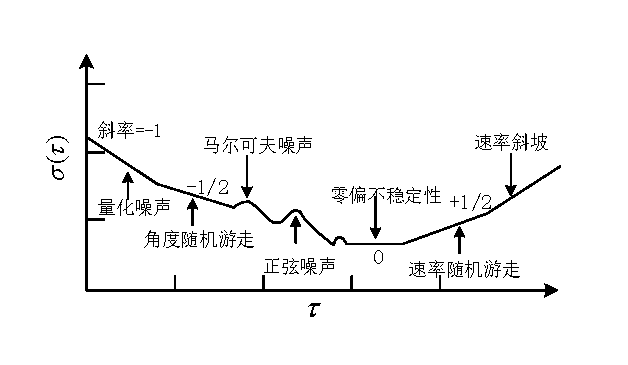
\includegraphics[width=0.5\textwidth]{figures/chapter2/fig2_12}
	\caption{Allan方差分析图}\label{fig2_12}
\end{figure}

首先区分几个比较复杂的概念,在2.1.3小节中说的白噪声 $\mathbf{n}_w, \mathbf{n}_a $通常在IMU使用手册中被描述为角度随机游走和速度随机游走,这是因为对角速度(加速度)的白噪声进行积分就是角度随机游走(速度随机游走)。也有的IMU手册中叫角速度噪声密度和加速度噪声密度,甚至直接简称为噪声密度。

角速率随机游走就是2.1.3小节中说的bias(随机游走) $\mathbf{b}_{w} $。一般IMU手册上不直接给出bias,而是给出bias (in)stability,即零偏(不)稳定性。因为在实践中,bias在长时间的积分中不会表现出真正的随机游走特性。bias (in)stability的值可以近似地表示bias的精度。在实践中,可以根据白噪声的大小以及bias (in)stability的值来确定bias的合理值。

Allan 方差可以分析任何信号,以确定潜在噪声过程的特征。信号的Allan方差是平均时间的函数。对于平均时间 $t$ ,Allan方差计算如下:

(1)获取一长串数据并将其按时间分成  $n$ 个长度为  $t$ 的区间。$n \geqslant 9 $ (否则得到的结果开始失去其意义)。

(2)求取每个区间中的数据的平均值得到平均值列表 $\left(a(t)_{1}, a(t)_{2}, \ldots, a(t)_{n}\right) $ 。 

(3)通过下面的式子计算Allan方差: 
\begin{equation}
\label{eqn:2.72}
\setlength{\abovedisplayskip}{6pt}
\setlength{\belowdisplayskip}{6pt}
\operatorname{AVAR}(t)=\frac{1}{2 \cdot(n-1)} \sum_{i}\left(a(t)_{i+1}-a(t)_{i}\right)^{2}
\end{equation}

为了分析噪声特性,需要计算Allan标准差:
\begin{equation}
\label{eqn:2.73}
\setlength{\abovedisplayskip}{6pt}
\setlength{\belowdisplayskip}{6pt}
\mathrm{AD}(t)=\sqrt{\mathrm{AVAR}(t)}
\end{equation}

在对数标度上绘制Allan标准差曲线(对数-对数AD曲线)。不同类型的随机噪声过程导致具有不同梯度的斜率。此外,不同的随机噪声过程通常出现在 $t$ 的不同区域中,从而可以容易地分辨出他们。确定随机噪声过程之后,可以直接从图中读取其数值参数。对于需要的白噪声,bias(随机游走)以及bias instability(零偏稳定性)可以通过下面的方式读取:

 (1) 对数-对数AD曲线上出现白噪声的地方的斜率为-1/2,通过在斜率上拟合直线并在$t=1$ 处读取。
 
 (2) 对数-对数AD曲线上出现bias(随机游走)的地方的斜率为+1/2,通过在斜率上拟合直线并在$t=3$ 处读取。
 
 (3) 对数-对数AD曲线上出现bias instability(零偏稳定性)的地方是曲线最小值附近的平坦区域,通过读取曲线上的最低点得到。

在IMU静止状态下采集四个小时的数据,然后绘制陀螺仪和加速度计的Allan方差曲线,如图\ref{fig2_13}和图\ref{fig2_14}所示。并将分析结果展示在表\ref{tab2.5}中,其中Gyr\_n和Acc\_n表示噪声项,Gyr\_w和Acc\_w表示随机游走。
\begin{figure}[!h]\setlength{\belowcaptionskip}{-12pt}
	\centering
	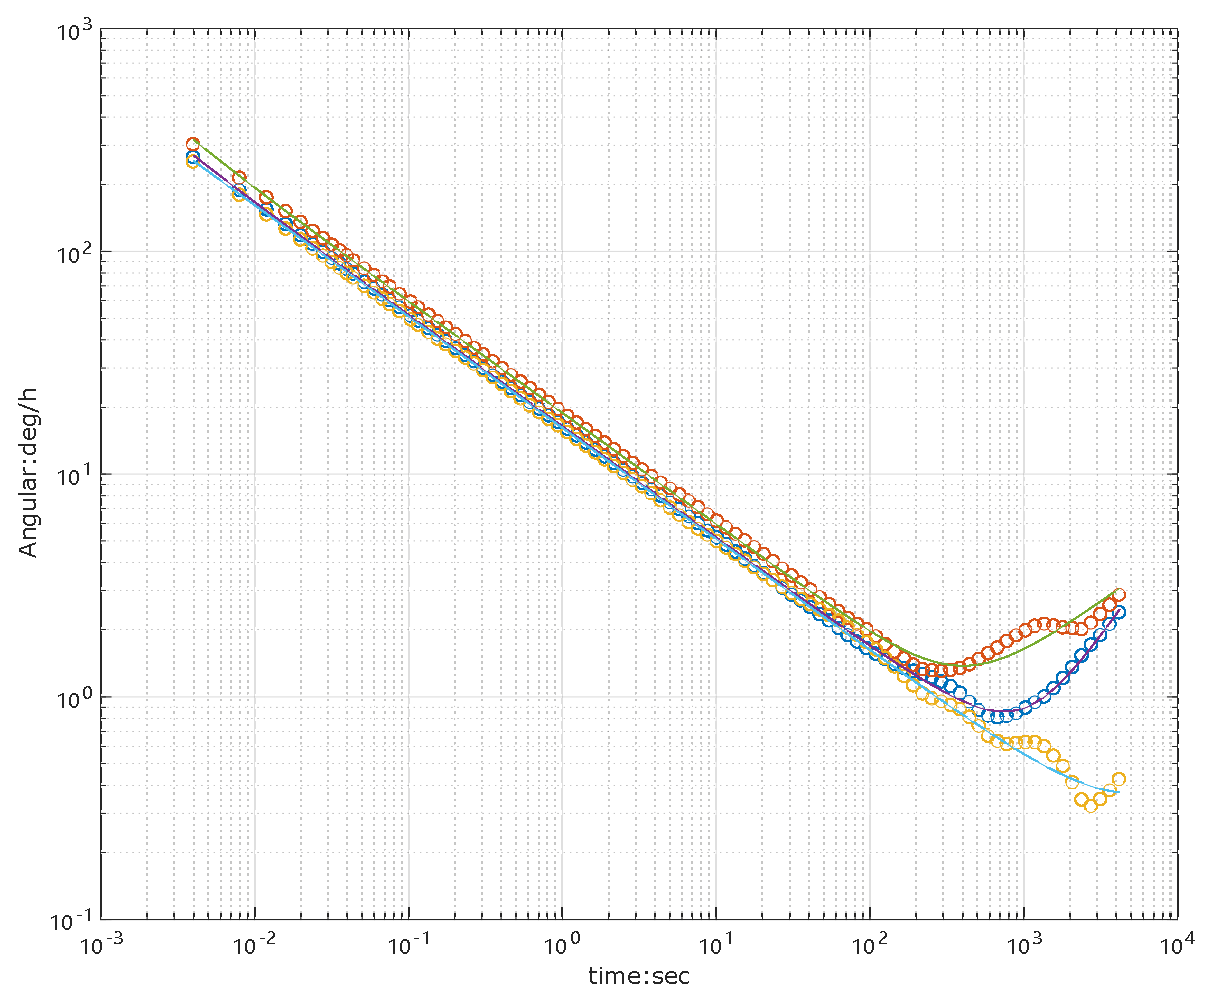
\includegraphics[width=0.8\textwidth]{figures/chapter2/fig2_13}
	\caption{陀螺仪Allan方差曲线}\label{fig2_13}
\end{figure}

\begin{figure}[!h]\setlength{\belowcaptionskip}{-12pt}
	\centering
	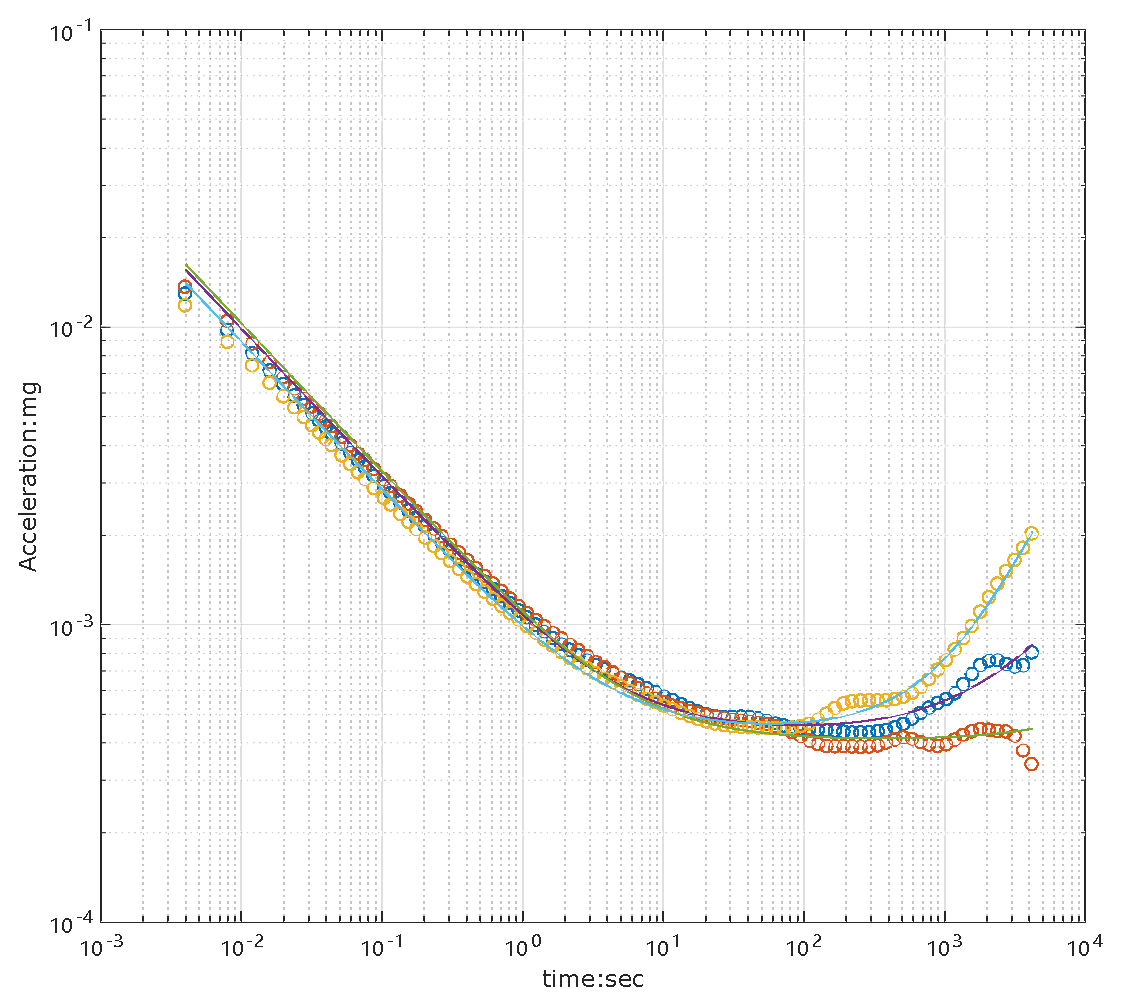
\includegraphics[width=0.8\textwidth]{figures/chapter2/fig2_14}
	\caption{加速度计Allan方差曲线}\label{fig2_14}
\end{figure}
\begin{table}[h]\setlength{\abovecaptionskip}{6pt}
	\zihao{5}  
	\centering
	\caption{IMU标定结果} \label{tab2.5}
	\begin{tabular*}{0.9\textwidth}{@{\extracolsep{\fill}}ccccc}
		\toprule
					&X轴		&Y轴	  &Z轴	&平均值 \\
		\midrule
		Gyr\_n (rad/s)	&1.25251e-03	&1.44058e-03	&1.23255e-03	&1.30854e-03\\
		Gyr\_w (rad/s)	&4.15778e-06	&6.66752e-06	&1.79872e-06	&4.20800e-06\\
		Acc\_n ($m/s^2$)	&1.70161e-02	&1.74575e-02	&1.56289e-02	&1.67009e-02\\
		Acc\_w ($m/s^2$)	&4.58804e-04	&4.14023e-04	&4.63646e-04	&4.45491e-04\\		
		\bottomrule
	\end{tabular*}
\end{table}
\subsection{同步与联合标定}
在视觉和IMU融合系统中,保证二者在时间上的同步非常重要。因为在初始化的时候需要将IMU预积分的值与视觉的观测值进行对齐,从而恢复单目视觉的尺度、重力的方向以及其它初始化参数。只有保证了正确的初始值,才能确保后端非线性优化能够收敛到一个最优值。而IMU和视觉对齐的程度完全取决于时间戳的匹配精准度。为了尽可能的对齐相机和IMU的时间戳,对传感器进行硬件同步。

本文选用的灰点相机拥有外部触发模式,也就是能够通过外部脉冲来触发相机进行曝光。选用的IMU能够向外输出与自己等采样频率的方波。如图\ref{fig2_15}所示,进行硬件同步的思路是:将IMU输出的方波(250Hz)通过硬件分频电路十分频,然后送到相机的触发端口(25Hz)进行触发曝光。

硬件同步为接下来的相机/IMU联合标定奠定了基础。
\begin{figure}[h]\setlength{\belowcaptionskip}{-12pt}
	\centering
	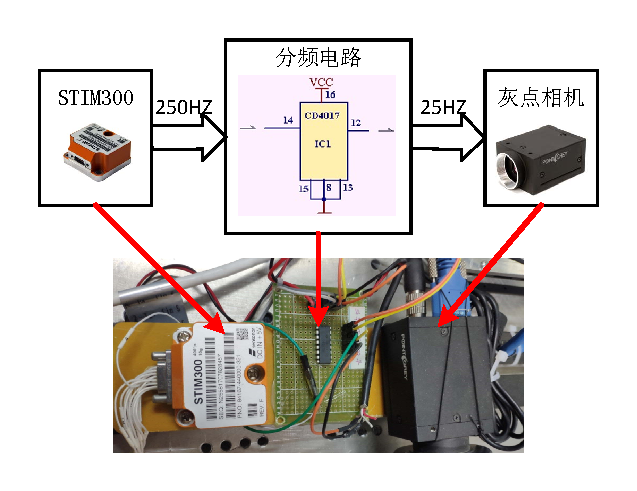
\includegraphics[width=0.45\textwidth]{figures/chapter2/fig2_15}
	\caption{硬件同步示意图}\label{fig2_15}
\end{figure}

使用开源的视觉/惯性标定工具:kalibr\upcite{furgale2012continuous}\upcite{furgale2013unified}进行联合标定。联合标定需要动态标定,需要的输入文件包括:相机内参及畸变参数,IMU噪声参数,带IMU信息的视频以及标定板信息。其中,相机内参和IMU噪声参数是\ref{chap:2.2.1}和\ref{chap:2.2.2}小节标定出来的结果。视频是在不同角度下拍摄的标定板图像,需要注意的是,在拍摄视频时需要激活IMU所有的轴向信息(包括偏航、横滚和俯仰)。采用的标定板和传统标定相机的棋盘格标定板(图\ref{fig2_11})不一样,是Aprilgrid标定板,如图\ref{fig2_16}所示。Aprilgrid标定板能够给出序号信息,可以避免姿态计算出现跳跃的情况。视IMU坐标系和载体坐标系重合,相机和IMU的坐标系定义如图\ref{fig2_17}所示。
\begin{figure}[h]\setlength{\belowcaptionskip}{-12pt}
	\centering	
	\begin{minipage}[t]{0.35\linewidth}				
		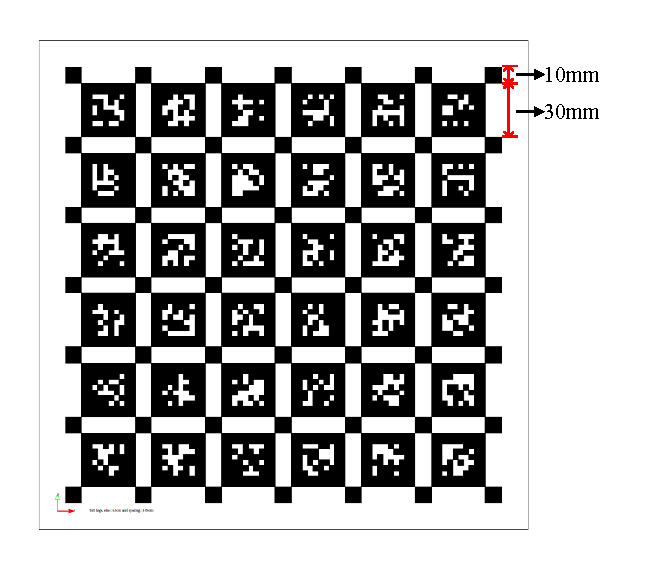
\includegraphics[height=4.5cm,width=6cm]{figures/chapter2/fig2_16}		
		\caption{Aprilgrid标定板}	\label{fig2_16}	
	\end{minipage}%	
	\hspace{0.1in}	
	\begin{minipage}[t]{0.5\linewidth}		
		\centering		
		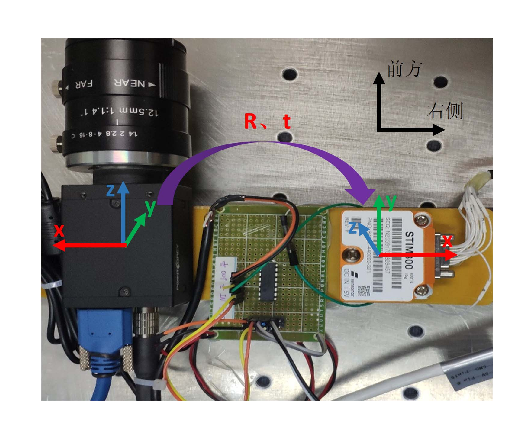
\includegraphics[height=4.5cm,width=6.5cm]{figures/chapter2/fig2_17}		
		\caption{相机和IMU的坐标系定义} \label{fig2_17}		
	\end{minipage}	
\end{figure} 

联合标定主要标定如下参数:

(1)  T\_ic:与IMU的外参。即相机到IMU的变换矩阵。

(2)  tmeshift:相机与IMU之间的时间偏移。这个值可以反应出时间同步的精度,timeshift越小表明同步效果越好。

(3)  Gravity vector:重力矢量。重力的大小能够反映出标定的精度。

另外,kalibr还会给出加速度和角速度的误差图,用来评估IMU的精度,以及相机重投影误差,可以用来评估的标定结果。

表\ref{tab2.6}是的相机和IMU联合标定的结果。可见相机和IMU之间的平移在10cm左右,这符合本系统实际安装距离。时间偏移约为9ms。重力大小是9.8$m/s^2$ 。可见,标定出的结果较为可靠。
\begin{table}[h]\setlength{\abovecaptionskip}{6pt}
	\zihao{5}  
\newcommand{\tabincell}[2]{\begin{tabular}{@{}#1@{}}#2\end{tabular}}  %导言区
	\centering
	\caption{联合标定结果} \label{tab2.6}
	\begin{tabular*}{0.75\textwidth}{@{\extracolsep{\fill}}cc}
		\toprule
		T\_ic			& $\left[ \begin{array}{cccc}
			0.99956 & 0.02956 & 0.00015 & 0.10048 \\ 
			 0.00028 & -0.00458 & -0.99999 & 0.01208 \\ 
			-0.02955 & 0.99955 & -0.00459 & -0.07922 \\ 
			{0} & {0} & {0} & 1
		\end{array}\right]$\\
		\midrule
		\tabincell{c}{Timeshift(s)}            &   -0.009307066448628993 \\
	    \midrule
		\tabincell{c}{Gravity vector($m/s^2$)}            &   [ 0.12538627\ \  -9.80181878\ \   -0.27757847] \\
		\bottomrule
	\end{tabular*}
\end{table}

图\ref{fig2_18}是IMU角速度误差和加速误差。可见,角速度误差在±0.04$rad/s$ 范围内波动,加速度误差在0.5$m/s^2$ 范围内波动。

图\ref{eqn:2.19}是相机的重投影误差。可见,重投影误差在±0.8个像素单位波动。这表明相机内参和畸变参数标定的很准确。
\begin{figure}[!h]\setlength{\belowcaptionskip}{-12pt}
	\centering
	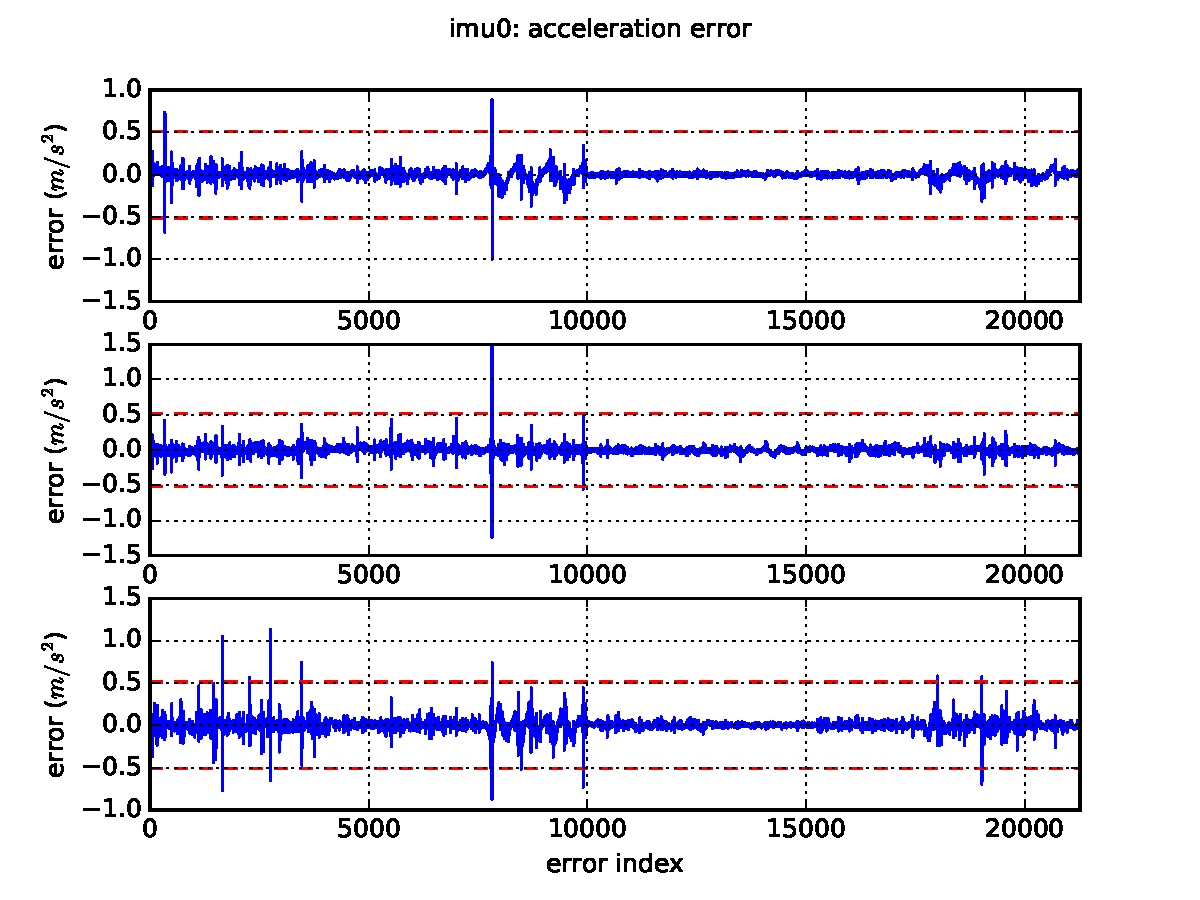
\includegraphics[width=0.47\textwidth]{figures/chapter2/fig2_18(a)}
	\hspace{0.01cm}
	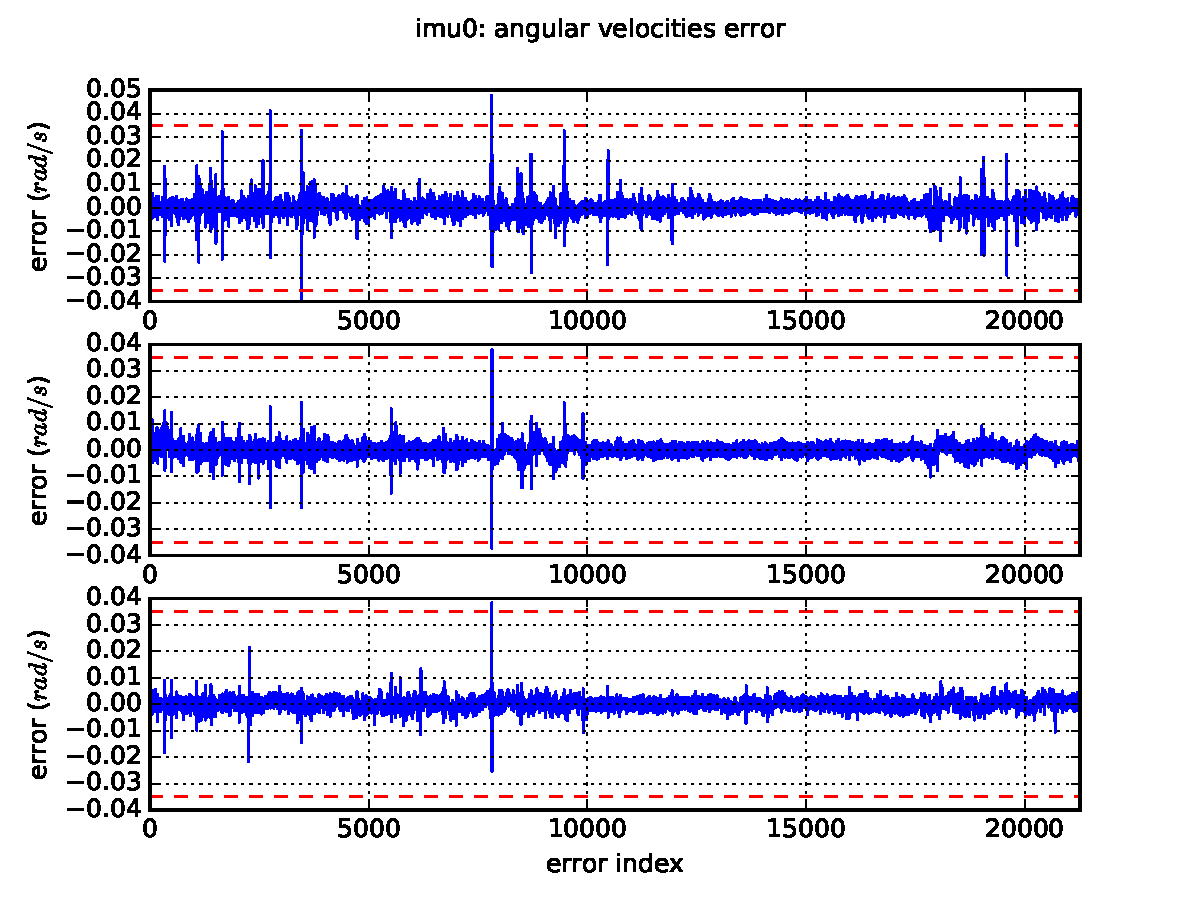
\includegraphics[width=0.47\textwidth]{figures/chapter2/fig2_18(b)}
	\caption{IMU角速度误差和加速误差}
	\label{fig2_18}
\end{figure}
\begin{figure}[!h]\setlength{\belowcaptionskip}{-12pt}
	\centering
	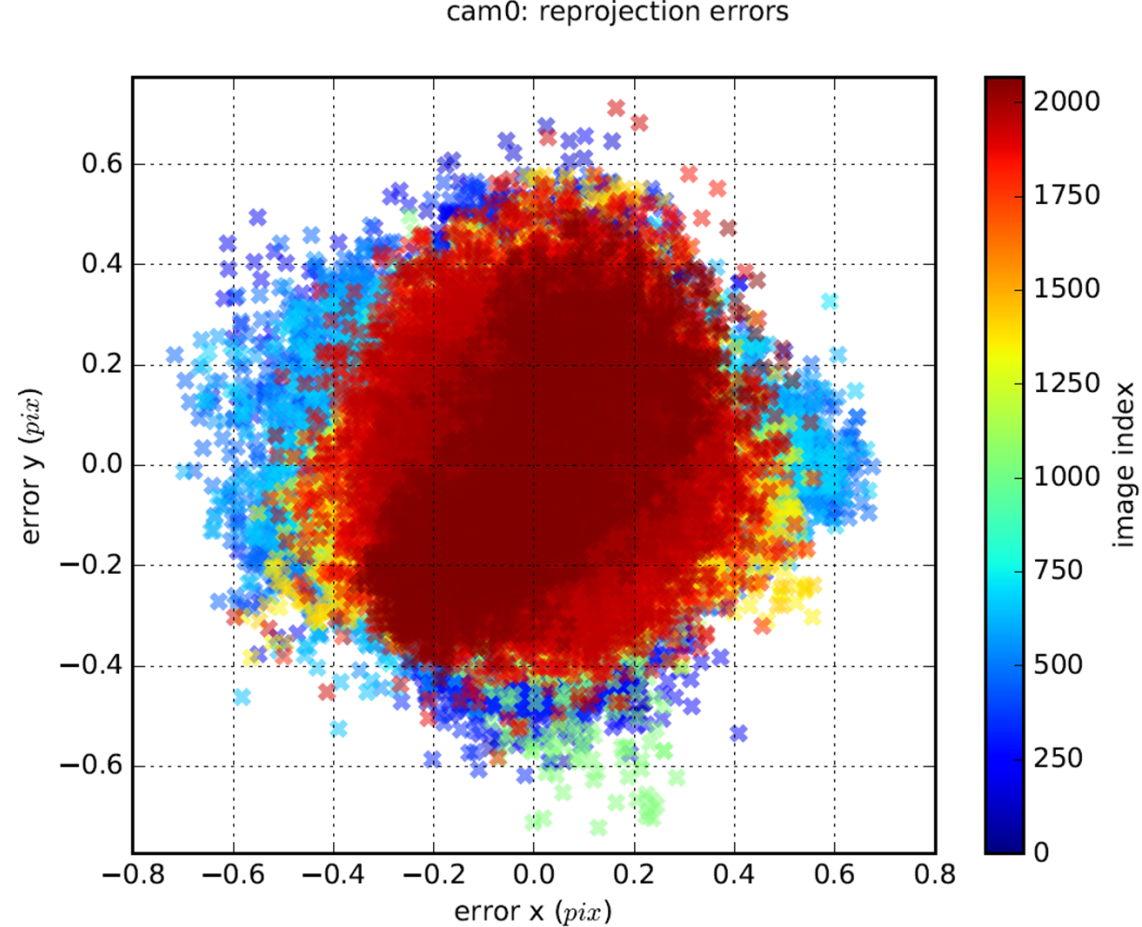
\includegraphics[width=0.6\textwidth]{figures/chapter2/fig2_19}
	\caption{相机重投影误差}\label{fig2_19}
\end{figure}
\section{硬件组建与ROS信息采集}
\subsection{硬件组建}
本系统的硬件系统构成如图\ref{fig2_20}所示。
\begin{figure}[h]\setlength{\belowcaptionskip}{-12pt}
	\centering
	\includegraphics[width=0.6\textwidth]{figures/chapter2/fig2_20}
	\caption{硬件系统构成}\label{fig2_20}
\end{figure}

图中\mycircled{1}是灰点单目相机(配镜头),\mycircled{2}是IMU(STIM300),\mycircled{3}是磁力计,\mycircled{4}是RTK,\mycircled{5}是12v锂电池,\mycircled{6}是稳压模块,\mycircled{7}是RS232串口转USB,\mycircled{8}是相机和IMU的同步电路,\mycircled{9}是Intel NUC处理器,\mycircled{10}是磁力计和底座连接的连接杆,\mycircled{11}是底座。其中,RTK不属于多传感器融合系统,主要用他来采集差分GPS信号,将GPS的轨迹当作真实值并和本系统输出轨迹作比较,方便分析系统的定位精度。为了避免载体(汽车)本身对磁力计的干扰,将磁力计用\mycircled{10}架高,相对于底座的高度为60cm。而且为了尽量避免铁磁性物体对磁场的干扰,硬件系统的底座以及连接杆都是铝制的。
\subsection{ROS信息采集}
ROS(Robot Operating System)译作机器人操作系统\upcite{Fairchild2016ROS},通常应用在机器人上,它操作简单,功能强大,尤其适用于向机器人这种多任务、多节点的复杂环境。ROS的功能非常丰富,本文不打算一一介绍,只对其通信机制中的“话题”作简要研究。

在ROS中,一个节点(Node)就是一个可执行文件。由于机器人的模块众多,通常不会将所有的模块放在一个节点中实现,而是一个节点实现一个模块。比如,节点1用来驱动相机获取图像,节点2用来驱动电机控制机器人移动,节点3用来接收图像并进行定位……这样以来可以降低系统的崩溃频率,使程序便于维护。
在ROS的众多通信方式中,话题(topic)是最常用的一种。话题适合处理类似传感器信息这样的实时性、周期性的消息。话题是一种节点与节点之间的单向异步通信方式。发布节点(Publisher Node)发布话题到节点管理器Master,订阅节点从Master订阅话题。订阅节点接收到话题消息后会触发回调函数,在回调函数里对话题消息进行处理。

如\ref{fig2_21}所示,使用节点1采集相机图像,话题为/camera/image\_raw;节点2采集IMU数据,话题为/imu\_data;节点3采集磁力计数据,话题为/dmc\_data;节点4采集RTK数据,话题为/rtk\_data。节点5,6,7分别代表前端、后端和回环。节点1$\sim$ 4采集到的传感器数据将被以话题的形式发布到节点管理器Matser,然后节点5,6,7都可以独立的订阅所有话题,并在自己的回调函数进行处理,各个节点互不干扰,独立运行,这就是话题单向异步通信的优势。值得称赞的是,使用ROS采集传感器信息的时候可以将所有话题记录下来,之后可以像回放视频那样重复播放,达到重复使用数据的效果。
\begin{figure}[h]\setlength{\belowcaptionskip}{-12pt}
	\centering
	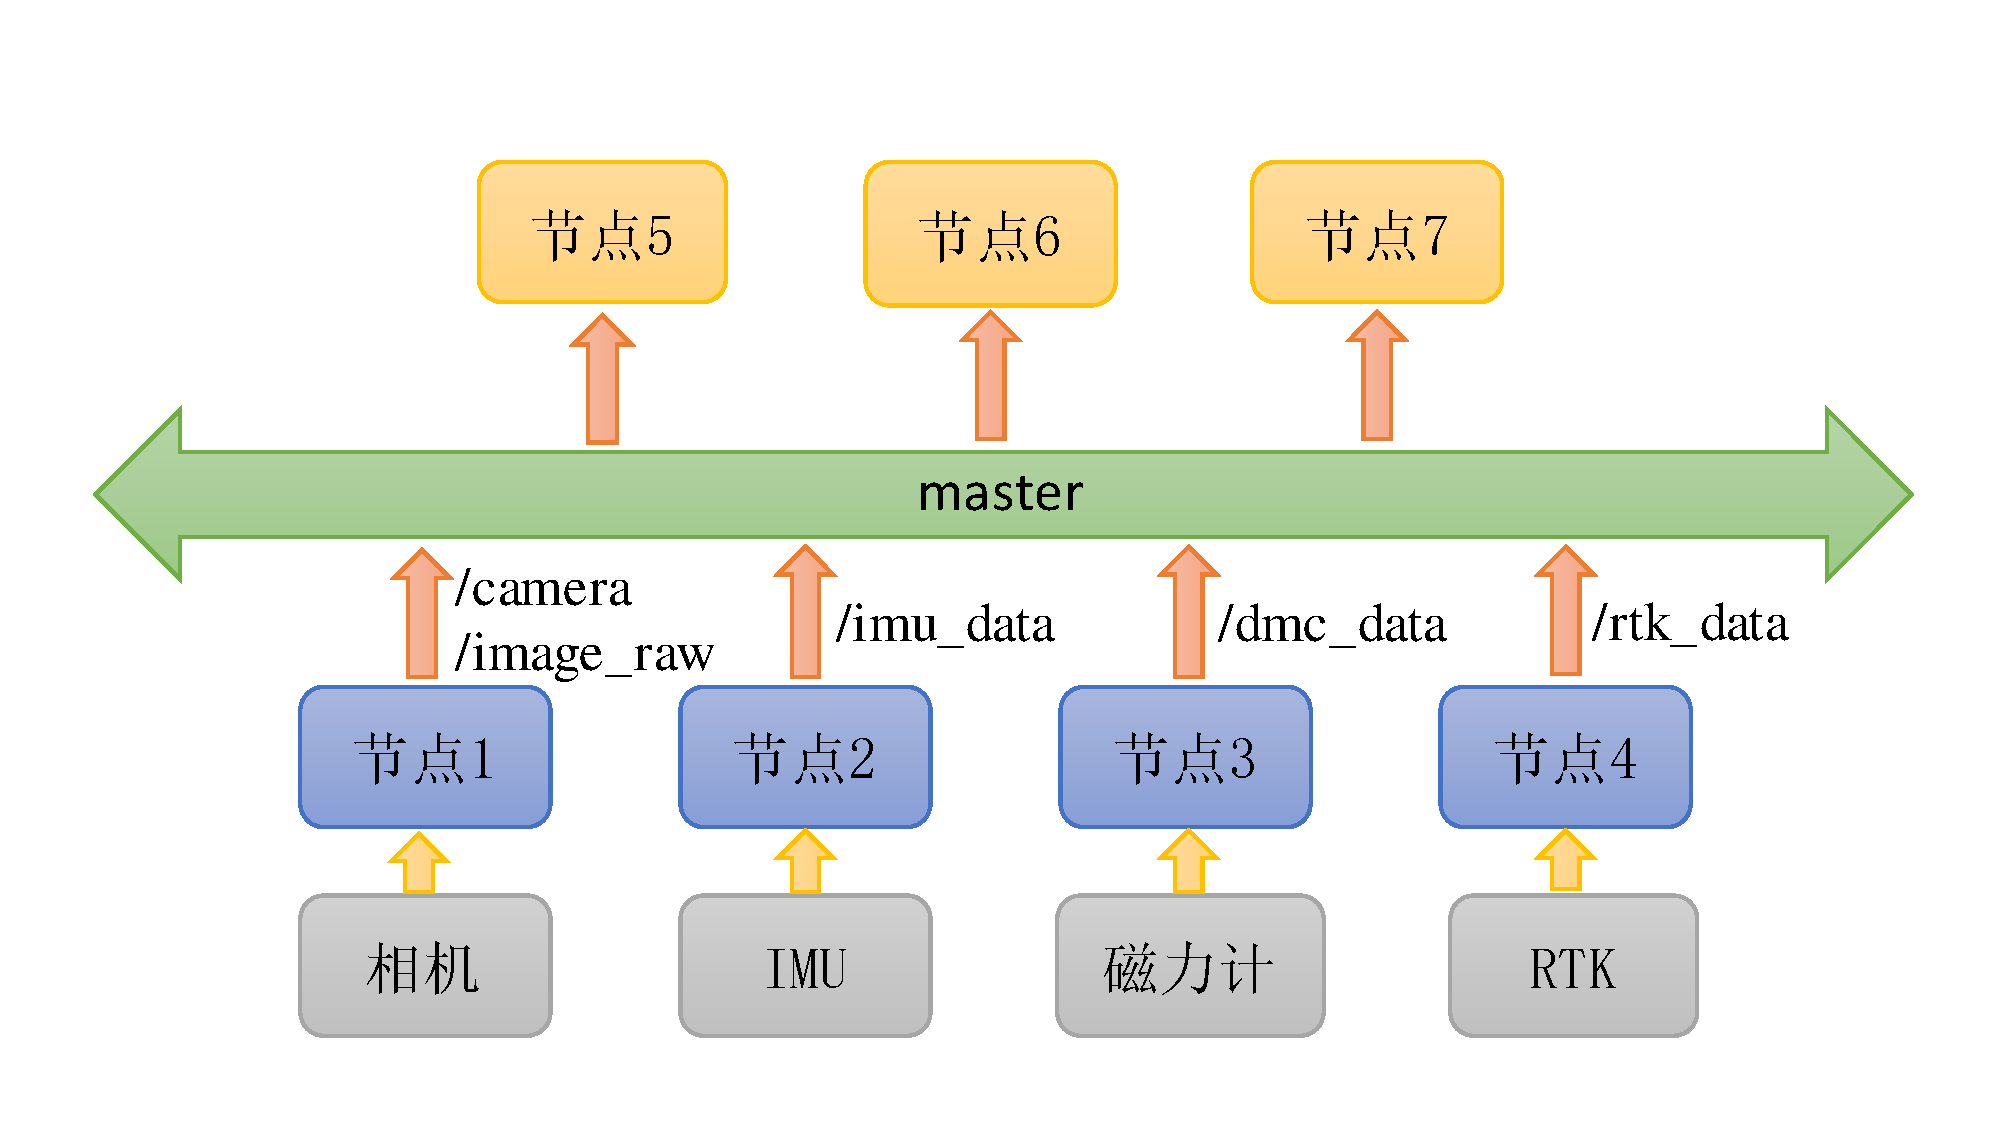
\includegraphics[width=0.6\textwidth]{figures/chapter2/fig2_21}
	\caption{ROS采集传感器信息及同通信示意图}\label{fig2_21}
\end{figure}
\section{本章小结}
本章主要研究系统的硬件部分,包括传感器模型及其选型,传感器标定与同步,以及硬件系统搭建和传感器信息采集。对传感器的数学模型进行了详细的推导,并详细研究了传感器的标定原理和步骤。完善可靠的硬件系统是后续进行算法研究和实验验证的基础。